\documentclass[12pt,a4paper]{article}
\usepackage[utf8]{inputenc}
\usepackage[english]{babel}
\usepackage{amsmath}
\usepackage{amsfonts}
\usepackage{amssymb}
\usepackage{latexsym}
\usepackage{makeidx}
\usepackage{graphics}
\usepackage{lmodern}
\usepackage{hyperref}
\usepackage{subcaption}
\usepackage{pgfplots}
\usepackage{dsfont}
\usepackage{multicol}
\usepackage{xcolor}
\usepackage{booktabs}
\usepackage{float}
\usepackage{subcaption}
\pgfplotsset{width=10cm,compat=1.9}
\usepgfplotslibrary{external}
\usepackage{graphicx}
\usepackage{wrapfig}
\author{Daniel Vázquez Lago}
\usepackage{fancybox}
\title{Apuntes Física Cuántica I}


\graphicspath{ {Imagenes/} }


\numberwithin{equation}{section}
\numberwithin{figure}{section}


\setlength{\parindent}{15px}
\usepackage[left=2.25cm,right=2cm,top=4cm,bottom=2cm]{geometry}


\newcommand{\parentesis}[1]{\left( #1  \right)}
\newcommand{\parciales}[2]{\frac{\partial #1}{\partial #2}}
\newcommand{\pparciales}[2]{\parentesis{\parciales{#1}{#2}}}
\newcommand{\ccorchetes}[1]{\left[ #1  \right]}
\newcommand{\D}{\mathrm{d}}
\newcommand{\derivadas}[2]{\frac{\D #1}{\D #2}}
\newcommand{\sech}{\mathrm{sech} \ }
\newcommand{\csch}{\mathrm{csch} \ }
\newcommand{\cotanh}{\mathrm{cotanh}}
\newcommand{\cotan}{\ \mathrm{cotan}}
\newcommand{\Res}{\mathrm{Res}}
\newcommand{\Arg}{\mathrm{arg}}
\newcommand{\Real}{\mathrm{Re}}
\newcommand{\tquad}{\quad \quad \quad}
\newcommand{\intf}{\int_{-\infty}^{\infty}}
\newcommand{\tint}{\iiint}
\newcommand{\rn}{\mathbf{r}}
\newcommand{\pn}{\mathbf{p}}
\newcommand{\kn}{\mathbf{k}}
\newcommand{\vn}{\mathbf{v}}
\newcommand{\Jn}{\mathbf{J}}
\newcommand{\Rn}{\mathbf{R}}
\newcommand{\Sn}{\mathbf{S}}
\newcommand{\Ln}{\mathbf{L}}
\newcommand{\qn}{\mathbf{q}}
\newcommand{\zn}{\mathbf{\hat{z}}}
\newcommand{\yn}{\mathbf{\hat{y}}}
\newcommand{\xn}{\mathbf{\hat{x}}}
\newcommand{\nmu}{\boldsymbol{\mu}}
\newcommand{\Bn}{\mathbf{B}}
\newcommand{\En}{\mathbf{E}}

\newcommand{\eup}{\mid \uparrow \rangle}
\newcommand{\edw}{\mid \downarrow \rangle}

\newcommand{\rota}{\nabla \times}
\newcommand{\dive}{\nabla \cdot}



\newtheorem{theorem}{Teorema}[section]
\newtheorem{corollary}{Corolario}[theorem]
\newtheorem{lemma}{Lema}[section]
\newtheorem{ejemplo}{Ejemplo}[section]

\begin{document}

\maketitle

\newpage

\tableofcontents

\newpage

\section{Pequeñas nociones matemáticas}

\subsection{Espacio de Hilbert}

Un espacio de Hilbert es un espacio vectorial equipado con un producto interno, que es una operación que toma dos vectores y devuelve un número complejo. En general describimos nuestro producto escalar con el siguiente simbolismo:

\begin{equation}
\langle \cdot | \cdot \rangle
\end{equation}

tal que debe verificar ciertas propiedades. Sean $x$, $y$, $z$ tres vectores (que en nuestra física cuántica serán operadores, es decir, ``funciones''):

\begin{itemize}
\item Linealidad:

\begin{equation}
\langle \alpha x + \beta y | z \rangle = 
\langle \alpha x | z \rangle + 
\langle \beta y | z \rangle
\end{equation}

\item Conjugado simétrico:

\begin{equation}
\langle x | y \rangle =  \overline{\langle y | x \rangle}
\end{equation}

\item Positividad:

\begin{equation}
\langle x | x \rangle \geq 0
\end{equation}
\end{itemize}

En la teoría cuántica el espacio de funciones será $L^2$, es decir, los vectores serán funciones de cuadrado sumable. En este espacio, el producto interno se define como la integral del producto de dos funciones (como una convolución de fouerier), y la norma se relaciona con la cuadrado-integrabilidad de las funciones.

\subsection{Matrices Hermiticas}

Definimos \textbf{matriz hermítica} o \textbf{matriz autoadjunta} $A$ como una matriz compleja que es exactamente igual que su conjugada traspuesta. Denotamos la matriz conjugada traspuesta como $A^\dagger$, de tal forma que:

\begin{equation}
A^\dagger_{ij} = \overline{A}_{ji}
\end{equation}

donde $\overline{A}_{ij}$ es el elemento conjugado en la fila $i$ columna $j$ de la matriz A. Nótese que cambiamos el orden de $ij$ a $ji$, lo que denota la condición de matriz transpuesta. En el contexto de la mecánica cuántica, las matrices hermíticas son particularmente importantes porque los operadores físicos que representan observables que deben ser hermíticos. Esto se debe a que las observables en mecánica cuántica deben tener valores reales, y las matrices hermíticas garantizan esta propiedad. Además, las matrices hermíticas tienen propiedades útiles en la diagonalización y descomposición espectral de operadores lineales. \\

Como este último punto es sumamente importante repasaremos un momento las definiciones de autovalores y autovectores para que no quepa ningún tipo de duda. \\

Un \textbf{autovalor} ($\lambda$) es un escalar (si hablamos de matrices complejas puede ser complejo) que verifica que para un vector $\vn$:

\begin{equation}
A \vn = \lambda \vn
\end{equation}

El \textbf{autovector} es el vector $\vn$ para el que existe un autovalor $\lambda$.  De esta forma cada autovector tiene su autovalor asociado. Con este primer trazado ya podemos vislumbrar un poco lo que se pretende: un operador cualquiera no será mas que una matriz en el espacio de Hilbert, y un autovector no será mas que un autoestado (ya lo veremos mas adelante) de tal modo que cualquier operador se pueda reducir a una suma de vectores o autoestados; donde el autovalor será el observable medible en el laboratorio. De hecho la razón por la que los operadores tienen que ser hermíticos es trivial si conocemos las propiedades de una matriz hermítica, que son:

\begin{itemize}
\item Todos los autovalores de una matriz hermítica son reales positivos, aunque la matriz sea compleja.
\item Todos los autovectores son ortogonales. Es decir, si no comparte el mismo autovector el producto escalar entre estos será cero.
\end{itemize}

de tal modo que nuestros medibles serán siempre positivos (es obvio que el cuadrado del momento lineal no puede ser negativo).

\newpage

\section{Principio de mínima acción}

Consideremos un cuerpo que se mueve en una dimensión sometido a cierto potencial $U(x)$. La Lagrangiana definida como $L=T-U$ nos permite, en la mecánica clásica, describir el movimiento de un objeto de manera \textit{unívoca} dadas unas condiciones iniciales (velocidad y posición para un tiempo $t_0$) siendo capaz de predecir la posición y velocidad del objeto en cualquier momento del tiempo futuro y conocer donde se ubico en el pasado. Entonces para un movimiento unidimensional la trayectoria $x(t)$ que debe seguir el cuerpo vendrá dada por:

\begin{equation}
\derivadas{}{t} \pparciales{L}{\dot{x}} - \parciales{L}{x} = 0
\end{equation}
que es la ecuación diferencial que minimiza la \textbf{integral de acción} $S$ definida como:

\begin{equation}
S = \int_{t_1}^{t_2} L(x(t),\dot{x}(t),t) \D t
\end{equation}

No obstante esta integral puede expresarse de múltiples formas. Como sabemos podemos definir el Lagrangiano como la diferencia entre energía cinética y la energía potencial. Sin embargo si tenemos en cuenta que $E = T + U$ podemos expresar el lagrangiano en función de la energía total (E) y la energía cinética, tal que

\begin{equation}
L = T - U = 2 T - E 
\end{equation}
Ahora bien, sabemos que $T = \frac{p^2}{2 m}$, y también sabemos que el momento $p = m (\D x / \D t)$. $x$. Si tenemos en cuenta esto y lo substituimos en la ecuación de la acción:
\begin{equation}
S = \int_{t_1}^{t_2} L(t) \D t =  \int_{x_1}^{x_2} p(x) \D x   - \int_{t_1}^{t_2} E \D t  = 
\end{equation}
Definimos al primer término de la integral como la \textbf{integral de acción reduica}, \textbf{acción reducida} o \textbf{acción característica}, nombrada por $S_0$, tal que

\begin{equation}
S_0 \equiv  \int_{x_1}^{x_2} p(x) \D x 
\end{equation}
En ese caso tendremos que si $\Delta t = t_2 - t_1$ y $E$ es una constante (por el principio de conservación de la energía podemos suponerlo) obtenemos que

\begin{equation}
S = S_0 - E \Delta t \longleftrightarrow S_0 = S + E \Delta t
\end{equation}
La acción reducida tiene una propiedad muy interesante que no debe pasar desapercibida por el lector:  tiene la propiedad de permanecer \textit{invariante} bajo cualquier redefinición del cero de la energía potencial. Además es una magnitud definida \textit{positiva}. Jugará un papel fundamental en el movimiento oscilatorio de los cuerpos.

\newpage



\section{La constante de Planck}

Como es fácilmente deducible la integral de acción es una cantidad medible en el laboratorio, solo es necesario conocer la la velocidad (o energía cinética) y posición en diferentes intervalos del tiempo, intentando causar la mínima perturbación posible sobre la partícula. Las leyes de la Mecánica Clásica no nos impiden medir cantidades \textit{todo lo pequeñas que queramos} por lo que podemos obtener la integral sin ningún tipo de problema. \\

Sin embargo la naturaleza, la realidad física, dice que esto no es posible. En realidad la integral de acción es una \textit{cantidad no nula y discretiza, da}, discretizada en múltiplos enteros de la constante de Planck. La continuidad del espacio y del tiempo a muy pequeña escala queda en entredicho, sin tener a día de hoy una respuesta muy clara. Lo que es claro es que la acción reducida \textit{sí} esta discretizada, con repercusiones en todas las ramas de la física.  \\

No obstante tomar la discontinuidad de la acción reducida como un postulado fundamental de la física no es suficiente para crear una nueva mecánica consistente y predictiva. Dicho hecho debe ser parte de la nueva mecánica, la \textit{mecánica cuántica}. Describimos este hecho con el siguiente principio: \\


\textbf{Principio de cuantificación de la acción:} \textit{Para cualquier observación física de un cuerpo o sistema de ellos, sometidos a un campo de fuerzas o de una onda sujeta al principio de mínima acción, ambos durante un tiempo $\Delta t$, la acción reducida $S_0$, extendida al intervalo $\Delta t$, sólo puede tomar valores que sean múltiplos enteros de la constante de Planck. La cuantificación tiene lugar en la forma:}

\begin{equation}
S_0 = (n+\alpha) h \tquad n=1,2,\ldots,\infty; \quad \alpha > -1
\end{equation}
\textit{donde $\alpha$ es una constante real específica para cada problema. Por ejemplo para el movimiento de un electrón alrededor de un núcleo atómico (regido por el potencial de Coulomb $\beta/r$) se cumple que $\alpha =0$.}. \\

Decimos que un objeto o un cuerpo se mueve en el \textbf{límite clásico} si $S_0 \gg h$ o que se mueve en el \textbf{límite cuántico} si $S_0 \simeq h$. Siempre que un cuerpo se mueva en el límite clásico podremos estudiar su movimiento según las leyes de la mecánica clásica. Sin embargo en el límite cuántico estas leyes dejarán de tener toda validez. \\

Una de las consecuencias mas interesantes de la discretización de la acción reducida es que cuando tratamos de calcular el valor medio de la energía cinética de una partícula en un tiempo $\Delta t$ cada vez mas pequeño (es decir, con mayor precisión) esta energía cinética tiende a aumentar, de tal manera que el aumento $\Delta \varpropto \Delta t^{-1}$. Este fenómeno se le conoce como \textbf{fluctuación cuántica}, y es responsable de la creación de pares de partículas-antipartículas virtuales. \\

A continuación vamos a estudiar el fenómeno del movimiento periódico. Para ello primero vamos a introducir un teorema fundamental, no solo en este tema, si no en los temas siguientes. Es común escribir la constante de Planck como $\hbar$ tal que:

\begin{equation}
\hbar = \dfrac{h}{2 \pi}
\end{equation}

\subsection{Movimiento periódico}

\begin{theorem}[Teorema del Virial]
sea  $\bar{T}$ la energía cinética promedio y $\bar{U}$ el potencial promedio. Si el potencial es un potencial central del tipo $U(r) =  \beta r^d$ con $d>-2$ entonces tenemos que la energía cinética promedio puede expresarse en función de la energía potencial como:

\begin{equation}
\bar{T} = \dfrac{d}{2} \bar{U}
\end{equation}
\end{theorem}

Esto tiene unas consecuencias colosales, ya que en este caso tenemos que la energía total se puede expresar en función del potencial como:

\begin{equation}
E = \parentesis{\dfrac{d+2}{2}} \bar{U}
\end{equation}
y la acción reducida puede expresarse como

\begin{equation}
S_0 = \bar{L} \Delta t = \parentesis{ \dfrac{2d}{(d+2)}} E \Delta t \label{Ec:03.4}
\end{equation}

No es trivial ver la relación que tiene esto con un movimiento periodico, pero trataremos de explicarla. Lo primero que debemos pensar es ¿Energía promedio \textit{de qué}? Es decir ¿En qué promedio estamos evaluando la energía? Esta es exactamente la pregunta que debemos hacernos, y no puede ser ahora, mas trivial: si el movimiento es un movimiento periódico está claro que el promedio será el \textit{periodo de la órbita}. Entonces queda claro que $\Delta t$ es el \textit{periodo de la órbita}. De esta forma podremos evaluar si un objeto se mueve en el límite clásico o cuántico: solo tendremos que evaluar este producto. \\

Es común además que el periodo tenga una relación uno a uno con la energía, siendo la excepción la del oscilador armónico ($d=2$). En el caso de un potencial con $d=-1$ tenemos por ejemplo que el periodo viene dado por la tercera ley de Kepler:

\begin{equation} 
\Delta t = \dfrac{\pi}{\sqrt{2}} \dfrac{\beta m_r^{1/2}}{|E|^{3/2}} \equiv \dfrac{2 \pi}{\omega}
\end{equation}
donde $m_r$ es la masa reducida. En la órbita de dos cuerpos con masas $m_1,m_2$ está está definida como:

\begin{equation}
m_r = \dfrac{m_1 m_2}{m_1 + m_2}
\end{equation}

A partir de estas ecuaciones vamos a calcular con precisión el tamaño de los átomos y el radio de Bohr. 

\subsection{Tamaño de los átomos y radio de Bohr}

Comencemos el estudio con el átomo de Hidrógeno, donde supondremos que tiene $Z$ protones para hacerlo mas general. Suponemos entonces que el único potencial que ve el átomo viene dado por el potencial de Coulomb, que vieen dado por $U(r) = - \beta /r$, con $\beta = \frac{Ze^2}{4 \pi \varepsilon_0}$. En ese caso tenemos que:

$$ S_0 = - 2 E \Delta t $$
aplicando la tercera Ley de Kepler
$$ S_0 = - 2 \dfrac{\beta m_r^{1/2}}{\sqrt{2} E^{1/2}} $$
Supongamos entonces que nos movemos en el ámbito cuántico, de tal manera que $S_0 = n h $ con $n=1,2,...$ En ese caso tendremos que la energía vendrá discretizada, de tal manera que:

\begin{equation}
E_n = - \dfrac{1}{2} \dfrac{m_r \beta^2}{\hbar^2} \dfrac{1}{n^2}
\end{equation}
Ahora la pregunta que falta es: ¿Podemos obtener un valor para el radio? La respuesta es no, de hecho la misma pregunta es errónea. No podemos afirmar con rotundidad, en un primer lugar, que ``orbite'' alrededor del núcleo. Lo único que sabemos es que tiene un movimiento periódico. De hecho la ecuación que rige el movimiento del electrón (estudiada en temas posteriores) no se parece en absoluto a una elipse. Además al ser $\Delta t \approx h/T$, las fluctuaciones cuánticas serán importantes. \\

En ese caso ¿Estamos condenados a no conocer el tamaño del átomo? La respuesta es no, y en realidad es muy sencilla. Precisamente la cuántica nos dice que la trayectoria mas probable es la trayectoria clásica. Por tanto podemos obtener una distancia para la cual encontrar el electrón es la mas probable. Para obtenerla usamos el teorema del virial, que nos dice que $E = U(r)/2$. Consecuentemente la distancia mas probable para cualquier energía $E_n$ vendrá de despejar $U(r)$ respecto $E_n$. En ese caso para el valor fundamental de la energía (el primer valor) obtenemos el \textbf{radio de Bohr}

\begin{equation}
a_0 = \dfrac{\beta}{- 2 E_1} = \dfrac{\hbar^2}{Z} \dfrac{4 \pi \varepsilon_0}{m_r e^2}
\end{equation}

Esto nos permite asignar valores para los casos de $Z=1$,$m_r = m_e$. En ese caso tenemos que $E_1 = -13.6 \ eV$ y que $a_0 = 0.0529 \ nm$. Como se puede ver cuando $n \rightarrow \infty$ tenemos que la diferencia relativa entre $E_{n+1}$ y $E_n$ es prácticamente nula, y por tanto podemos decir que pasamos a valores casi continuos, propio del límite clásico. \\

Al contrario de lo que se dice, el estado de mínima energía no proviene del equilibrio entre las fuerza de Coulomb (atracción) y la fuerza centrífuga (repulsión). Esto no es verdad, porque el electrón no orbita. En realidad el equilibrio de fuerzas se origina de la pérdida de energía por radiación (atracción) debida a la ley de Larmor y el aumento de energía cinética debido a las fluctuaciones cuánticas, ya que al acercarse su mayor localización temporal hace que aumente drasticamente la energía cinética (repulsión). El equilibrio hace entonces que la distancia mas probable sea el radio de Bohr $a_0$   \\

\subsection{Densidad de niveles de energía}

Este tema es fundamental para entender el tema \ref{Sec:24}. Si es la primera vez que se lee podéis sin lugar a dudas saltaros este tema, no os va a aportar nada hasta llegar a ese tema, aunque trataré de hacerlo lo mas comprensible posible. Por lo pronto si no habéis entendido nada de dicha sección revisitar este tema puede ser clave. \\

Supongamos que estamos en un espacio de $N$ dimensiones por lo que designamos a la posición como $q_i$ y el momento $p_i$ para cada dimensión. Entonces la integral de acción de un movimiento periódico  (donde hemos hecho que $p^2 /2m = p v$ y que $v \D t = \D x$, suponiendo 

$$ S_0 = \oint  \pn \D \qn = \sum_{i=1}^N \oint p_i \D q_i = \sum_{i=1}^N S_0^i = \sum_{i=1}^N (n_i + \alpha_i) h $$

Ahora si aplicamos el teorema de Green $\oint p_i \D q_i = \iint \D p_i \D q_i = (n_i + \alpha_i) h$. Entonces el área encerrada por la trayectoria en el espacio $(qi, pi)$ es aproximadamente un múltiplo $n_i$ de un cuadrado elemental o píxel $\delta q_i \delta p_i$ de área h. Por tanto todo el volumen en el espacio fásico puede ser aproximado por un volumen $h^N$.  \\

Definimos entonces $\Omega (E)$ como el valor del volumen del espacio fásico para un nivel de energía determinado. Como sabemos la energía depende del momento (o el momento de la energía) por lo que tendremos que limitar la integral de momentos. Para esto usamos la función $\theta(x)$ de Heavside definida como:

\begin{equation}
\theta (x) = \left\lbrace \begin{array}{ll}
0 & \quad \mathrm{si} \ x<0 \\
1 & \quad \mathrm{si} \ x>0 
\end{array} \right.
\end{equation}
de tal manera que

\begin{equation}
\Omega (E) = \int \D^N q \int \theta (E-H(\qn,\pn)) d^N p
\end{equation}
tal que $\theta = 1$ siempre que $E>H$, lo cual tiene todo el sentido del mundo. No tendría sentido evaluar la integral en valores donde $H>E$. De cualquier modo, definimos entonces el \textbf{número promedio de niveles de energía} como:

\begin{equation}
\langle \mathcal{N} (E) \rangle \equiv \Omega (E) / h^N
\end{equation}
ya que nos da el número de pixeles que hay en el espacio fásico del problema en cuestión para cierta energía. Es muy interesante además la \textbf{densidad promedio} de niveles por unidad de intervalo de energía, tal que:

\begin{equation}
\langle \D  \mathcal{N} / \D E \rangle \equiv (\D  \Omega / \D E) / h^N
\end{equation}
Este valor será muy interesante de calcular en intervalos donde $(E,E + \Delta E)$ con $\Delta E$ pequeño en comparación con $E$ pero grande para el espaciado promedio de niveles. \\

Un problema donde podemos aplicar este es el problema de 3 dimensiones donde encerramos una partícula libre en un volumen $V$. En ese caso tenemos que 

$$ \Omega(E) = V \cdot 4 \pi \int \theta(E - p^2/2m) p^2 \D p = \dfrac{4 \pi}{3}  V \parentesis{2mE}^{3/2}  $$

\newpage


\section{Propagación de Fenyman}

Es el carácter discreto y no nulo de la acción reducida el que permite que existan las fluctuaciones cuántica. Esto no es coinciliable con una física de trayectorias diferenciables. Si intentamos imaginarnos el movimiento como una sucesión de pequeños intervalos llegaremos a la conclusión de que las trayectorias realmente no son diferenciables, ni siquiera seremos capaces de predecir con exactitud la posición de una partícula en un instante conocido un instante y posición anterior: es remotamente imposible, ya que va saltos. \\

Entonces quedan claras dos cosas: la nueva formulación del a física no debe ser determinista, no podemos conocer, con unas condiciones iniciales dadas, las posiciones de una partícula en instantes posteriores; pero también se debe cumplir que en el límite clásico se recuperen las leyes clásicas. ¿Como podemos juntar estas dos? Para no abandonar las trayectorias diferenciales lo que haremos será asumir que la \textit{partícula se mueve por todas las trayectorias posibles}.  \\


La formulación de la física cuántica, la nueva física, nos obliga a admitir que todas las posiciones intermedias de la partícula son posible y que la partícula recorre todas las trayectorias posibles a la vez. Para precisar este concepto Feynman desarrollo la \textbf{amplitud de propagacion} $K(x,t) \equiv \langle \ x \ t \ | \ x_1 \ t_1 \ \rangle$ como un número complejo que caracteriza el movimiento desde el punto $x_1$ al punto $x$. \\

 Ahora bien ¿Por qué un número complejo? Un número complejo viene dado por dos partes, un módulo y una fase. La fase nos permite hacer que ciertas posiciones interfieran entre sí, de tal modo que se vayan cancelando las partes. En general un número complejo actúa como una función oscilatoria, por lo que si dos posiciones están en desfase total se cancelarán entre sí. Está claro que la trayectoria clásica debe ser la que mas influencia tenga, ya que de otro modo si llevamos el caso a tiempos ``humanos'' no obtendríamos las trayectorias que vemos. Entonces a medida que nos alejemos de la trayectoria clásica habrá mas osiclaciones (en la fase) de tal forma que en entre dos puntos infinitamente cercanos habrá una oscilación, cancelando la influencia de ambos en el movimiento. \\
 
Para cualquier intervalo de tiempo la amplitud de propagación para la transición entre dos puntos satisface que: 

\begin{equation}
\langle x_2 \ t_2 | x_1 \ t_1 \rangle = \int_{-\infty}^{\infty} \langle x_2 \  t_2 | x \  t \rangle \cdot \langle x \ t | x_1 \ t_1 \rangle \D x
\label{Ec:3-Postulado-Propagación}
\end{equation}

que es el llamado \textbf{postulado de Propagación} de Feynman. Ahora tenemos que definir cual es la operación que rige a $K(x,t)$. La definición matemática tiene que solucionar un punto: tiene que haber interferencias entre los posibles caminos para que en límites macroscópicos se verifiquen las leyes de Newton. Para esto usaremos una función oscilatoria dada por un número complejo. 

\begin{equation}
K(x,t,x_1,x_2) \equiv \langle x \ t \ | \ x_1 \  t_1 \rangle = A e^{\frac{i S}{\hbar}} = \sqrt{\frac{m}{i 2 \pi \hbar \Delta t}} \exp \ccorchetes{\dfrac{m (x-x_1)^2}{2 \Delta t} - U \parentesis{\frac{x+x_1}{2},t} \Delta t}
\label{Ec:3-Principio-Propagación}
\end{equation}

A este se le llama el \textbf{principio de propagación} de Feynman. Esta idea de que la amplitud se construye como la suma de muchos caminos distintos que contribuyen simultáneamente al movimiento se llama principio de superposición, y se resume diciendo: ``para moverse de un punto a otro los cuerpos deben sondear antes  todas las posiciones del espacio, y tendrán mas influencia aquellas mas cercanas al movimiento clásico''. En la Mecánica Clásica determinista esta amplitud sería uno para la trayectoria definida por las ecuaciones de Euler-Lagrange y cero para el resto. Una de las manifestaciones de este principio se da en los experimentos de la doble rendija. \\




Dudas: ¿A que se refiere con la frase "para moverse de un punto a otro los cuerpos deben sondear antes  todas las posiciones del espacio, y tendrán mas influencia aquellas mas cercanas al movimiento clásico"?

\section{Velocidad Instatánea}

Debido a las fluctuaciones cuánticas no podemos definir un concepto como el de velocidad instantánea (solo promedio) por lo que toda la diferenciabilidad de las trayectorias se rompe indudablemente. \\

Esta es una conclusión en última instancia del carácter discreto de la acción reducida ha que cuando tratamos de observar la partícula durante intervalos de tiempo cada vez mas cortos la energía cinética aumenta y por lo tanto el cociente $\Delta x / \Delta t \rightarrow \infty$. 

\section{Ecuación de Schrödinger}

Matemáticamente hablando resulta mas sencillo resolver una ecuación diferencial que realizar el cálculo de las ecuaciones \ref{Ec:3-Postulado-Propagación} y \ref{Ec:3-Principio-Propagación}. La ecuación diferencial que nos permite calcular $K(x,t)$ es la famosa \textbf{ecuación de Schrödinger}:

\begin{equation}
i \hbar \parciales{K(x,t)}{t}  = \dfrac{- \hbar^2}{2 m} \parciales{^2 K(x,t)}{x^2} + U(x,t)K(x,t)
\end{equation}

que es una ecuación diferencial compleja. Se puede escribir en forma de real de tal forma que tomemos la parte real del número complejo si $U(x,t) = 0$. En cualquier otro caso es completamente obligatorio usar números complejos.


\section{Función de ondas}

En la Mecánica Cuántica todo movimiento es posible. Por tanto una partícula que se encuentra inicialmente en un punto, en un espacio de tiempo ocupará virtualmente todo el espacio, y cada punto a su vez es susceptible de propagarse por todo el espacio. Por tanto se hace necesaria la definición de forma general el \textit{estado de ocupación del espacio} de una partícula en un momento determinado. \\

Tiene interés en conocer la amplitud total que tenga un partícula para llegar a un punto $(x,t)$ sin conocer el pasado, ya que realmente se puede encontrar en cualquier punto. A esta nueva ecuación la denotaremos por $\Psi (x,t)$, y la llamaremos \textbf{función de ondas}. No hay diferencia con el concepto de $K$. Como esta ecuación es válida para cualquier punto en el que se encuentre inicialmente (se puede encontrar en cualquier punto) entonces la ecuación de ondas debe satisfacer:

\begin{equation}
\Psi (x,t) = \int_{-\infty}^\infty K(x,t;x_1,t_1) \Psi (x_1,t_1) \D x_1
\end{equation}

En términos físicos: la amplitud total de ($x,t$) es la suma integral sobre todos los valores posibles de $x_1$, de la amplitud para llegar al punto $(x_1,t_1)$, multiplicada por la amplitud para llegar desde $x_1$ a $x$. Básicamente es como decir que multiplicas la probabilidad de que este en $x$ siendo $x_1$ cualquier punto (ya que lo estás integrando entre todos los $x_1$ posibles). En ese caso es fácil de demostrar la función de onda satisface:

\begin{equation}
i \hbar \parciales{\Psi}{t} = \parentesis{\dfrac{- \hbar^2}{2m} \parciales{^2}{x^2} + U(x,t)}\Psi
\end{equation}

Así pues la función de onda será una función compleja que nos define el estado de movimiento de un cuerpo en el tiempo t. Además tiene una interpretación probabilística ya que:

\begin{equation}
\intf |\Psi (x,t)|^2 \D x = 1
\end{equation}

La única condición para que esto sea de tipo \textit{cuadrado sumable}, es decir, que sea finita la integral entre menos infinito e infinito. Luego se podría normalizar sin mucha dificultad. Una propiedad muy importante es que cualquier redefinición de la energía potencial, tiempos o fase carece de significado físico y representa el mismo estado (tal que $U(x,t) \rightarrow U(x,t) + C$).

\section{Onda de De Broglie y transformación de Fourier}

Desde el punto de vista matemático, la ecuación de Schrödinger es una ecuación en derivadas parciales de segundo orden que contiene la derivada primero respecto el tiempo. Si el potencial es cero (movimiento libre), una posible solución es la onda plana:

\begin{equation}
\Psi (x,t) = A e^{i(kx-\omega t) } \label{Ec:7-ondaplana}
\end{equation}
donde $\omega$ debe ser exactamente

\begin{equation}
\omega (k) = \dfrac{\hbar k^2}{2 m}
\end{equation}
para que así verifique la ec. de Schrödinger. La onda plana de De Broglie es una representación ideal, de tal manera que no decae en el infinito, como ocurre en la realidad. Además ni siquiera es de cuadrado sumable (ya lo veremos) por lo que no pertenece al espacio de Hilbert que deben pertenecer las ecuaciones de ondas. Una de las hipótesis mas importantes de la física cuántica es la \textbf{hipótesis de De Broglie}, que nos dice que: \textit{todo cuerpo móvil con momento p lleva asociada una onda que es consustancial con su estado de movimiento y cuya longitud de onda vale}

\begin{equation}
\lambda = \dfrac{h}{p}
\end{equation}
\textit{siendo h la constante de Planck}. Esta es una de las ecuaciones mas importantes de la física ya que relaciona el momento de cualquier cuerpo con una longitud/número de onda, siendo esta onda nada mas que el estado definido por la ecuación de Schrödinger del cuerpo. \\


Definimos velocidad de grupo como $ v_g = \D \omega / \D k$ de tal forma que:

\begin{equation}
p = m v_g = \hbar k
\end{equation}

de lo que se deduce que

\begin{equation}
E = \dfrac{p^2}{2m} = \hbar \omega
\end{equation}

donde no solo es la energía cinética si no toda la energía de un cuerpo. En este caso relativista la onda no verifica la ecuación de Schrödinger vista si no su versión relativista. Una onda de estas características es fuertemente dispersiva, lo que se hace notar cuando superponemos ondas con distintos valores de $\lambda$ para formar un pulso, pues las velocidades de propagación sin inversamente propocionales a sus longitudes de onda. \\

Por lo tanto la solución de la ecuación como una onda plana es una idealización matemática ya que en la realidad no existen trenes de onda completamente monocromáticos, solo durante una longitud, la \textit{longitud de coherencia}, decayendo a cero fuera de ella. Esto equivale a decir que las partículas nunca tendrán su momento definido con total precisión. Los estados de onda plana no constituyen funciones de ondas de cuadrado sumable por lo que el valor de la constante $A$ \ref{Ec:7-ondaplana} en la ecuación no puede ser determinado por normalizar la integral. \\

Definimos la \textit{transformada de Fourier} de la función de ondas como:

\begin{equation}
f(k) \equiv \dfrac{1}{\sqrt{2 \pi}} \intf \Psi (x) e^{-ikx} \D x
\end{equation}

y el \textbf{teorema de inversión de Fourier} asegura que la función de ondas original en función de $x$ puede recuperarse usando:

\begin{equation}
\Psi (x) = \dfrac{1}{\sqrt{2 \pi}} \int_{-\infty}^{\infty} f(k) e^{ikx} \D k
\end{equation}

Lo anterior nos dice básicamente que cualquier ecuación de onda puede construirse como la suma de ondas planas con distintas longitudes de onda. Además de que las funciones $f(k)$ y $\Psi (x)$ proporcionan dos descripciones equivalentes de un mismo estado de movimiento, pues contienen exactamente la misma información. Ahora $|f(k)|^2 \D k$ estará asociado con la probabilidad de detectar un momento.

\section{Valores medios e indeterminación}

Ya que la función de ondas de una partícula ocupa todo el espacio es interesante conocer cual es la coordenada promedio de la posición, así como conocer si dispersión alrededor del valor medio. En resumen: queremos conocer la extensión espacial sobre la que la partícula fluctúa con mayor probabilidad. Viene dada por:

\begin{equation}
\langle x \rangle = \intf x |\Psi (x) |^2 \D x = \intf \Psi ^* (x) (x \Psi (x)) \D x
\end{equation}

\begin{equation}
\Delta x^2 = \langle x^2 \rangle - \langle x \rangle^2
\end{equation}
donde 

\begin{equation}
\langle x^2 \rangle = \intf x^2 |\Psi (x)|^2  \D x
\end{equation}

No siendo posible la definición de una velocidad instantánea (como ya hemos visto) pero si una velocidad promedio y un momento promedio. Al igual que la posición promedio de la partícula viene dada por la partícula por la función de ondas en $x$, el momento $k$ vendrá dado por $k$ con la función de ondas escrito en lenguaje momento. Entones el momento viene dado por:

\begin{equation}
\langle p \rangle = \hbar \langle k \rangle = \hbar \intf k |f(k)|^2 \D k = m \langle v \rangle
\end{equation}

Otra forma de calcular el momento teniendo que usar dos integrales (la primera para calcular la transformada de Fourier) es usar la definición de producto escalar de la transformada de Fourier dentro del conjunto de funciones de onda pertenecientes al espacio de Hilbert (básicamente es cualquier espacio donde está definido un producto escalar, sean funciones o vectores):

\begin{equation}
\langle \Psi_1 | \Psi_2 \rangle = \intf \Psi_1^* (x) \Psi_2 (x) \D x
\end{equation}
Además usando la \textit{identidad de Parseval}:
\begin{equation}
\intf  \Psi_1^* \Psi_2 \D x = \intf f_1(k) f_2^* (k) \D k
\end{equation}

Si aplicamos lo que es la transformadas de Fourier, usamos las propiedades y matemáticas vistas hasta ahora, seremos capaces de calcular nuestro momento $p$ (usando que $p = k \hbar$):

\begin{equation} 
\langle p \rangle = \intf \Psi^* (x) \parentesis{- i \hbar \parciales{\Psi}{x}} \D x
\end{equation}
eso podemos aplicarlo para cualquier magnitud física medible. Entonces todas las magnitudes físicas medibles (momento lineal, momento angular...) necesitan un operador definido de la función de ondas, que en general se denotará igual que el valor. El alumno deberá diferenciar de manera natural cuando se usa operador y cuando es una magnitud física medible. A partir de ahora llamaremos al \textbf{operador momento} el siguiente operador:

\begin{equation}
p = - i \hbar \parciales{}{x} 
\end{equation}
cada magnitud física tendrá ahora un operador asociado que se relacionará de alguna manera u otra con la función de ondas y los estados. No tienen otra finalidad que calcular valores medios, y se consideran aplicaciones lineales del espacio de Hilbert. Obviamente estos valores medios deben siempre reales por lo que los operadores físicos deben ser autoadjuntos, lo que implica una relación de estos operadores con las matrices complejas hermíticas (que son operadores lineales autoadjuntos sobre el espacio vectorial).  El \textbf{operador momento cuadrado} $p^2$ unidimensional, necesario para calcular posteriormente la energía cinética del operador $H$ de la ecuación de Schrödinger es:

\begin{equation}
p^2 = - \hbar \parciales{^2}{x^2}
\end{equation} 

Vemos entonces que el operador que aparece en la ecuación de Schrödinger $H$, que no es mas que la energía cinética mas la energía potencial (i.e. la energía total), no es mas que el operador en coordenadas unidimensionales:


\begin{equation}
H = - \dfrac{\hbar}{2 m} \parciales{^2}{x^2} + U(x,t)
\end{equation}

Ahora hemos aprendido a decodificar la información contenida en la función de ondas de una partícula para poder hacer predicciones estadísticas sobre los resultados de las medidas de cualquier observable en el laboratorio. Si estamos en un espacio con 3 dimensiones será ($\Delta \equiv \nabla^2$, laplaciano tridimensional):

\begin{equation}
H = - \dfrac{\hbar}{2m} \parentesis{\parciales{^2}{x^2}+\parciales{^2}{y^2}+ \parciales{^2}{z^2}} + U(\rn,t) = - \dfrac{\hbar}{2m}(\Delta + U(x,t))
\end{equation}


\section{Principio de Indeterminación}

El enunciado del \textbf{principio de indeterminación de Heisenberg} no tiene ninguna raíz física, es una deducción puramente matemática que viene de la definición de la transformada de Fourier. Este nos dice que si conocemos con gran precisión ($\Delta x$) la posición que ocupa un cuerpo entonces son inevitables grandes fluctuaciones en su momento ($\Delta p$), estando las anchuras de ambas distribuciones  relacionadas por la desigualdad:

\begin{equation}
\Delta x \Delta p \geq \hbar/2
\end{equation}

Su impacto es enorme, ya que revela la imposibilidad de conocer simultáneamente con infinita precisión la posición de un cuerpo a lo largo de una dirección determinada y su momento en esa misma dirección. Evidentemente podemos conocer con infinita precisión la posición de un cuerpo en una dirección y la del momento en otra dirección. Una consecuencia inmediata es que todo cuerpo confinado en una región del espacio (tamaño 2 $\Delta x$) adquiere una energía cinética con valor medio:

\begin{equation}
\langle T \rangle = \dfrac{1}{2 m} (\Delta p)^2 \geq \dfrac{1}{4} \dfrac{1}{2m} \dfrac{\hbar^2}{(\Delta x)^2}
\end{equation}

y cuando una partícula se desplaza con una velocidad de grupo en forma de un pulso dispersivo tiene sentido definir la \textit{indeterminación en el tiempo} ya que $\Delta t = \Delta x/ v_g$, de lo que se deduce el \textbf{principio de indeterminación del tiempo}

\begin{equation}
\Delta E \Delta t \geq \hbar / 2
\end{equation}


Es muy importante conocer la aproximación $\Delta x \Delta p \thicksim \hbar$ (para una dimensión) ya que nos permite calcular ciertos valores como la masa de una partícula o la energía de una partícula. Esta aproximación solo será válida sí: la partícula se encuentre cerca de su estado fundamental, la partícula no haya sido abandonada en movimiento libre. Si no se cumplen dicho producto será mayor que $\hbar$. \\

\section{Autoestados y autovalores}

Dada una magnitud física nos debemos preguntar si existen estados cuánticos que nos permitan definir bien dicho valor. Esto matemáticamente se traduce en: ¿Existen funciones de onda tales que una magnitud sea medible e unequívoca?. Otra pregunta que debemos hacernos es: ¿Se pueden medir en un espacio continuo dicha magnitud física?¿O por el contrario está discretizada?. \\

Para nosotros todo magnitud física medible, de ahora en adelante \textbf{observable}, tiene asociado un operador lineal. Vease el caso del operador momento, el operador momento al cuadrado o el operador Hamiltoniano. Este operador lineal no es otra cosa que una matriz en nuestro espacio de Hilbert $L^2$ (se que me repito mas que el ajo pero es que es sumamente importante este concepto) que está operando sobre un vector para obtener así otro vector en el espacio de Hilbert $L^2$. Entonces podemos plantear el problema como un problema de \textit{autovalores} y \textit{autovectores}. Entonces supongamos que somos capaces de encontrar los autovectores y autovalores del problema:

\begin{equation}
A \Psi = a \Psi
\end{equation}

Es decir, la matriz (operador) $A$ aplicado sobre el vector (función de ondas de cuadrado sumable) $\Psi$ es exactamente igual que un número real (medible) $a$ multiplicado escalarmente por dicho vector (función de ondas). Como para nosotros estos vectores son al fin de al cabo funciones de ondas que \textit{definen el estado de nuestro sistema} llamaremos a los autovectores \textbf{autoestados}. Como exigimos que $A$ es hermítico los autovalores siemrpe serán positivos y reales, lo que cuadran con un valor medible en la vida real. \\

Entonces todos aquellos valore reales de $a$ que no pertenezcan al espectro de autovalores resultarán prohibidos, y será imposible medirlos. Por esa razón la física es \textit{cuántica}. Además como los autovectores de una matriz hermítica son ortogonales (es decir su producto escalar es nulo) tenemos que los autoestados forman una base ortonormal de funciones, las \textbf{autofunciones}. Consecuentemente podemos definir cualquier estado, cualquier función de ondas, como la suma de autofunciones. \\

Un fenómoeno super curioso es el fenómeno del \textbf{colapso de ondas}. Supongamos que un cuerpo o partícula se encuentra en un estado $\Psi$ que no es un autoestado. Cuando vamos a medir un observable $a \in \mathbb{R}$ tenemos que la función de ondas experimenta un cambio: se transforma en la función $\Psi_a$ correspondiente al autovalor medido. Este fenómeno todavía desconocido manifiesta a la perfección el carácter no determinista de la mecánica cuántica, ya que el conocimiento de la función de ondas previa a la observación no nos permite conocer el valor medido a priori, ya que cambiará. Ese colapso de la función de ondas no está gobernada por la ecuación de Schrödinger. \\

Entonces cualquier función de ondas se puede escribir como:

\begin{equation}
\Psi ( \rn ) = \sum_n \sum_m c_{n,m} \Psi_{a_n,m} ( \rn )
\end{equation}

donde los coeficientes complejos $c_{n,m}$ se pueden calcular como productos escalares de tal forma que $c_{n,m} = \langle \psi_{a_n,m} | \psi \rangle$. El \textbf{coeficiente m} representa la multiplicidad de un autovalor: un autovalor puede tener diferentes vectores asociados ortogonales. Esto llevará a la degeneración cuántica y a la definición cuántica de la entropía. Llamamos a $m$ la degeneración de un estado cuántico solo para el caso de la multiplicidad de la energía. Para visualizarlo mejor podemos estudiar el caso del momento angular dentro de un átomo: para un mismo momento angular $l=0,1...n-1$ asociado a un nivel de energía podemos encontrar hasta $2l-1$ electrones tal que sus funciones de onda son completamente ortogonales. \\

La propiedad de normalidad exige que la suma de todos estos sea uno $\sum_{n,m} |c_{n,m}|^2 = 1$  y por lo tanto $P_n = \sum_m |c_{n,m}|^2$ determina la probabilidad de que la medida realizada sobre $\Psi$ arroje el valor $a$.\\

Otra forma de relacionar los autoestados es el uso de la transformada inversa de Fourier, ya que una integral de Riemann o integral es, al final, usa suma llevada al límite infenitesimal, de tal forma que:

\begin{equation}
\Psi (\rn) = \dfrac{1}{(2\pi)^{3/2}} \tint f(\kn) e^{i \kn \rn} \D ^3 \kn = \sum_{\kn} c_\kn e^{i \kn \rn}  = \sum_{n} c_{\kn_n} e^{i \kn_n \rn }
\end{equation}

Esta suma recorre el conjunto de autovalores $a_n = \pn_n = \hbar \kn_n$ correspondientes a las autofunciones ondas de De Broglie $e^{i \kn_n \rn}$ del operador momento. En este caso los coeficientes complejos $c_{\kn_n}$ no son mas que el producto escalar entre las autofunciones de onda de De Broglie, de tal forma que:

\begin{equation}
c_{\kn_n} = f(\kn_n) = \langle \Psi_{a_n} | \Psi \rangle = \langle e^{i \kn_n \rn} | \Psi \rangle
\end{equation}

\section{Estados estacionarios}


%Imaginemos una trayectoria clásica periódica de energía $E$, que se inicia en el punto $\rn_0$ con periodo $\Delta t$. En cada instante de tiempo la partícula ira recorriendo puntos, pudiendo asociar a cada uno de esos puntos el valor de la fase dado por la acción clásica completa en el propagador de Feymann:

%\begin{equation}
%K = A e^{iS/\hbar} = A e^{-iEt/\hbar}e^{iS_0/\hbar}
%\end{equation}

%Si queremos que el movimiento sea periódico es necesario que la acción reducida. La condición real de cuantificación de la acción reducida es:

%\begin{equation}
%S_0 / \hbar = (n + \mathcal{M}/4) 2 \Pi
%\end{equation}

%donde $\mathcal{M}$ es un número entero positivo llamado \textbf{índice de Maslov}. Esto permite que existan trayectorias periódicas en el movimiento, bien sea un movimiento integrable (N grados de libertad con N-1 constantes del movimiento) o un movimiento caótico (solo se conocen N grados de libertad con N-1 constantes del movimiento) o un movimiento caótico (solo se conserva E). Entonces la fórmula de la acción reducida vista anteriormente $S_0 = (n + \alpha ) h$ es una excelente aproximación para calcular las energías de un sistema integrable. \\

%Sin embargo nosotros no queremos una aproximación: queremos conocer la solución exacta para el problema de las energías.

Un movimiento periódico puede ser integrable (solo se conocen N grados de libertad con N-1 constantes del movimiento) o caótico (solo se conserva E). Sea cual sea podemos suponer que existen estados de energía bien definido, donde el factor de fase de $e^{-iEt/\hbar}$ del propagador de Feynman es heredado por la función de ondas. Debemos conocer exactamente el problema de las energías, y para ello usaremos la ecuación de Schrödinger. Como la función de ondas de una partícula debe presentar en todos los puntos del espacio una fase común, por lo que deseamos que la densidad de probabilidad de encontrar una partícula en cualquier punto $\rn$ sea constante en el tiempo:

\begin{equation}
\parciales{| \Psi (\rn,t)|^2}{t} = 0 \label{Ec:11.044}
\end{equation}

es decir hemos descrito una densidad de probabilidad estacionaria. Para lograr encontrar una solución a la ec. de Schrödinger debemos realizar los siguientes pasos:

\begin{itemize}
\item Resolver la ecuación de autovalores para el operador energía $H$:

\begin{equation}
\parentesis{\dfrac{-\hbar^2}{2m} \Delta + U(\rn)} \Psi (\rn) = E \Psi (\rn)
\end{equation}

para algún valor de $E$ real. Además la función de ondas debe tener sentido, es decir: debe ser de cuadrado sumable y estar normalizada, además de que debe ser continuo en todo $\mathbb{R}^3$ que no sea un potencial infinito. Es el cumplimiento de estas dos condiciones, \textit{y no de la solución de la ecuación de ondas}, lo que restringe los valores de la energía a unos \textit{valores discretos}.

\item Construir una ecuación de ondas con la siguiente dependencia temporal:

\begin{equation}
\Psi (\rn,t) = e^{-i E t/\hbar} \Psi (\rn)
\end{equation}

que representa estos estados estacionarios, ya que verifica la ecuación de ondas y la condición \ref{Ec:11.044}. 

\end{itemize}

Entonces tenemos que nuestra ecuación de Schrödinger se ha convertido en una \textbf{ecuación de Schrödinger independiente del tiempo}:

\begin{equation}
H \Psi = E \Psi
\end{equation}

donde $H$ es un operador y $E$ autovalores. Su solución conlleva una ecuación diferencial de segunda orden independiente del tiempo, siendo necesarias ciertas condiciones de contorno. Hablar de una ecuación independiente del tiempo es análogo a hablar de una función de ondas donde la incertidumbre del tiempo es infinita $\Delta t \rightarrow \infty$ y por tanto la energía está inequívocamente definida $\Delta E \rightarrow 0$. La ecuación de ondas en una dimensión queda en una dimensión como:

\begin{equation}
\parentesis{- \dfrac{\hbar^2}{2m} \parciales{}{x^2} + U(x)} \Psi (x) = E \Psi (x) 
\end{equation}




 Una vez resuelto el problema de la energía con un determinado potencial disponemos de un de un conjunto de autofunciones y autovalores de la energía. Este conjunto descrito como:

\begin{equation}
\lbrace \Phi_{n,m} (\rn), E_n,g_n,n=1,2...,m=1,2... \rbrace
\end{equation}

proporciona la solución exacta para los niveles de energía y su densidad que posee todo sistema físico periódicamente confinado. \\

Cualquier función puede representarse como la combinación lineal de autoestados de energía. Entonces:

\begin{equation}
\Psi (\rn,t) = \sum_n c_n e^{-i E_nt/\hbar} \Phi_n(\rn)
\end{equation}

es importante darse cuenta que una función descrita de esta forma no representa, en general, un estado estacionario. De hecho la única condición para que la energía este bien definida es que la partícula no se mueva. Si no se mueve (es decir el cuadrado de la función de ondas es constante en el tiempo) tenemos que la energía no cambiará con el tiempo y por lo tanto estará inequívocamente definida. De esto se deduce que \textit{todo movimiento se debe a la superposición de estados cuánticos}. Para entenderlo imaginemos un cuerpo con la energía definida de tal manera que $\Delta E = 0$. Por el principio de indeterminación tenemos que $\Delta t$. En otras palabras: el tiempo no existe para esta partícula, a partir de su estado no puedes concluir en que momento del tiempo está, no tiene sentido definir tiempo en este sistema. Solo la superposición de dos o mas funciones de ondas permite que exista el movimiento (cambio del cuadrado de la función de ondas respecto al tiempo) ya que exisitrá siempre un factor dependiente al tiempo asociado:

\begin{equation}
\Psi (r) = e^{i E_1 t} \Psi_1(\rn) + e^{i E_2 t}\Psi_2 (\rn)  \longrightarrow \parciales{ \Psi^{2}}{t} =  -2 E_1 E_2 e^{i (E_1 + E_2) t} \Psi_1 (\rn) \Psi_2 (\rn)
\end{equation}
El propagador de Feynman se puede escribir de manera exacta como:

\begin{equation}
K(\rn_1,t_1,\rn_2,t_2) = \sum_n \Phi_n (\rn_2) \Phi_n^* (\rn_1) e^{-i E_n (t_2-t_1)/\hbar}
\end{equation}

donde la suma se extiende sobre todos los estados estacionarios posibles del sistema. Una de las mas curiosas aplicaciones de que se pueda considerar que la función de ondas venga dada por $\Psi (\rn,t) = e^{- i E t/\hbar} \Psi (\rn)$ (y todas sus consecuencias) es que podemos determinar unequívocamente determinar la evolución temporal exacta de la función de ondas si conoces su valor inicial, tal que:

\begin{equation}
\Psi (t,t) = \mathcal{U}(t)  \Psi (\rn,0)
\end{equation}

donde hemos supuesto que hemos resuelto el problema de autovalores de la energía. Nuestro operador $\mathcal{U}(t)$ tendrá la siguiente forma de matriz diagonal:

\begin{equation}
\mathcal{U}(t)  = \mathrm{diag} \parentesis{e^{-i E_1 t / \hbar}, e^{-i E_2 t / \hbar, ...}}
\end{equation}

que representa, matemáticamente, la acción de las distintas frecuencias (recordemos que $E = \hbar \omega$) que originan el movimiento. Suponiendo que el problema de autovalores está resuelto tenemos que el operador Hamiltoniano $H$ es $H = \mathrm{diag} \parentesis{E_1,E_2,...}$. Por tanto relacionamos $\mathcal{U}$ con $H$: $\mathcal{U}(t) = e^{-iHt/\hbar}$. Para un estado cuántico, usando la notación de Dirac:

\begin{equation}
| \Psi (\rn,t) \rangle = \mathcal{U} (t) | \Psi (\rn,0) \rangle
\end{equation}

\section{Formulación de Bohr}

Como acabamos de ver si una partícula o cuerpo se encuentra definido por una combinación de dos o mas estados cuánticos esta partícula puede moverse. Supongamos ahora que solo está definido por dos estados, un estado $E_2$ y $E_1$ tal que $E_2 > E_1$. Esta situación es muy general, y se le llama \textbf{oscilación cuántica}. En función de las propiedades de dicha partícula. \\

Si nos fijamos en un punto $\rn$ del espacio tenemos que:

\begin{equation}
|\Psi (\rn,t)|^2 = |c_1|^2 |\Psi_1|^2 + |c_2||\Psi_2|^2 + 2 \Real \parentesis{|c_1 c_2|  |\Psi_1 \Psi_2| e^{-i( (E_2 - E_1)t/\hbar -\phi)}}
\end{equation}
donde $c_1$ es un número real y $c_2 = |c_2| e^{i \phi_0}$ siendo $\phi$ la fase relativa. Está claro que los valores oscilan entre un máximo $A+B$ y un mínimo $A-B$ tal que:

\begin{equation}
A(\rn) = |c_1|^2 |\Psi_1|^2 + |c_2||\Psi_2|^2 ;  \tquad B(\rn) = |c_1 c_2| |\Psi_1 (\rn) \Psi_2 (\rn)|
\end{equation}

La oscilación cesa en el momento que \textit{obligas} a la partícula a definirse por uno de los autoestados (cosa que ocurre cuando tratas de medirla). Durante la oscilación la energía no se encuentra bien definida, de tal manera que $\Delta E = |c_1 c_2 | (E_1 E_2)$. Cuando la partícula cae al estado más bajo de energía (no puede subir a no ser que le llegue un fotón externo) se emitirá un fotón con una frecuencia que seguirá la fórmula de Bohr:

\begin{equation}
E_2 - E_1  = \hbar \omega
\end{equation}
Esta ecuación es directamente deducida de la ec. de Schörodinger. 

\section{El momento angular}

Todo cuerpo que ocupe el punto $\rn$ con momento $\pn$ gira alrededor del origen siempre que no sean colineales. Dicho giro se conoce como \textit{momento angular} tal que $\Jn = \rn \times \pn$. Todo giro de un cuerpo se puede descomponer en dos: el giro alrededor de si mismo llamado \textit{espín} $\Sn$ y el giro alrededor de un punto externo llamado \textit{momento angular orbital}. En general: $\Jn = \Ln + \Sn$. Como su propia definición hace referencia al momento y a la posición podemos intuir que el principio de indeterminación tiene mucho que decir acerca de las limitaciones sobre sus medidas.\\

Como la función de ondas contiene toda la información sobre el estado de movimiento de un cuerpo, debe contener la información del momento angular. Los grados de libertad necesariamente cuánticos permiten describir su espín periten la aparición de distinas componentes $\Psi (\rn)$ de la función de ondas. \\

Como podemos intuir es imposible medir en el laboratorio sus 3 componentes y definir con total certeza sus componente total. De esto se deduce que \textit{el momento angular no puede proyectarse nunca íntegramente a lo largo de ningún eje}. Es fácil de ver si hacemos la reducción al absurdo: si $\Ln$ se orienta al eje Z, tenemos que $\rn$ y $\pn$ se orientan hacia el plano perpendicular al eje $Z$ (necesariamente), por lo que $\Delta z = 0$ y $\Delta p_z = 0$ cosa que es imposible. \\

Para toda función de ondas se debe verificar que $\Ln^2 > \Ln_z^2$ (o cualquier otro eje). Esta desigualdad es clave para entender el fenómeno del paramagnetismo, ya que el momento magnético individual no puede orientarse íntegramente a lo largo del campo magnético externo. \\

Ahora estudiemos el comportamiento del operador momento angular, ya que como toda cantidad medible en el laboratorio el cálculo del mismo debe implicar la definición de un operador momento angular. Conocido el operador posición y el operador momento tenemos que el operador momento angular se define como:

$$\Ln = \rn \times \pn = - i \hbar \rn \times \nabla $$
Es decir por cada componente se verificará que:

\begin{equation} 
L_x = - i \hbar \parentesis{y \parciales{}{z}-z\parciales{}{y}} \xn; \quad L_y = - i \hbar \parentesis{z \parciales{}{x}-z\parciales{}{x}} \xn; \quad L_z = - i \hbar \parentesis{x \parciales{}{y}-y\parciales{}{x}} \xn; 
\end{equation}

O lo que es lo mismo: el operador momento angular llevará implícito un rotacional. En general la formulación del operador momento angular se da en función de las coordenadas esféricas. Hay variar razones por las que se hace así: eliminamos una variable en las derivadas (solo derivará respecto las coordenadas angulares) y permite la posterior expresión en función de los armónicos esféricos, empleados en casi todas las ramas de la física. Entonces:

\begin{equation}
L_x = - i \hbar \parentesis{- \sin \phi \parciales{}{\theta} - \dfrac{\cos \phi}{\tan \theta}\parciales{}{\phi}}; \quad L_y  = - i \hbar \parentesis{{\cos \phi} \parciales{}{\theta} - \dfrac{\sin \phi}{\tan \theta} \parciales{}{\phi}}; \quad L_z = - i \hbar \parciales{}{\phi} \label{Ec:funcionesangulares}
\end{equation}
como obviamente el operador cuadrático vendrá dado por la misma relación trigonométrica que relaciona el momento total con cada una de sus partes ($L^2 = L_x^2 + L_y^2 + L_z^2$), tenemos que el operador $L^2$ es:

\begin{equation}
L^2 = - \hbar^2 \ccorchetes{\dfrac{1}{\sin \theta} \parciales{}{\theta} \parentesis{\sin \theta \parciales{}{\theta}} + \dfrac{1}{\sin^2 \theta} \parciales{^2}{\phi^2}} \label{Ec:funcionangularcuadrado}
\end{equation}


que es exactamente que la \textit{parte angular del operador de Laplace}. Entonces es obvio que podemos calcular el valor medio de $\Ln$ y $L^2$ así como su dispersión tal y como hemos visto en temas anteriores. \\

Ahora la experiencia sugeriría buscar algún tipo de solución por autovalores y autfunciones. Sin embargo ello obliga a estudiar 4 ecuaciones diferenciales, donde además será imposible encontrar una función de ondas para la cual se verifiquen las ecuaciones de $x,y,z$ por el principio de incertidumbre. Tampoco podemos decir que el conjunto de autovalores que encontremos sea diferente para cada eje ya que la elección de ejes es arbitraria. \\

En ese caso podemos encontrar que solo tiene sentido resolver simultáneamente las siguientes ecuaciones diferenciales:

\begin{equation}
L_z \Psi (\rn) = l_z \Psi (\rn) \tquad L^2 \Psi (\rn) = a^2 \Psi (\rn) \label{Ec:autoestadosmomentoangular}
\end{equation}

Como el operador $L_z$ es muy sencillo tenemos que la dependencia de $\Psi(\rn)$ respecto el ángulo $\phi$ debe ser del tipo $$ e^{i l_z \phi/\hbar}$$ donde claramente $l_z$ debe ser real de la forma $l_z =0, \pm \hbar, \pm 2 \hbar...$ es decir un múltiplo de la constante de plank. Es decir los estados para los cuales la partícula gira en el plano xy están cuantizados. \\

La razón detrás de dicha cuantización radica en que si la exponencial compleja no tuviera múltiplos de $\phi$ la función no podría ser univaluada, condición necesaria en nuestra compresión de la física cuántica (de momento). Solo la resolución detallada de las ecuaciones para $L^2$ nos pueden dar los valores de $|\Ln|$. La cuantificación es:

\begin{equation}
| \Ln | = 0, \sqrt{2} \hbar, \sqrt{6} \hbar, \sqrt{12} \hbar, \sqrt{20} \hbar, \ldots
\end{equation}
tal y como veremos en la siguiente sección.

\section{Autoestados del momento angular}

De ahora en adelante lo que haremos será intentar resolver la función de ondas para las condiciones \ref{Ec:autoestadosmomentoangular} tal que $l_z$, que luego se convertirá en $m$. Sin embargo nunca deberemos olvidar la naturaleza de este, que no es mas que los posibles estados de $l_z$, aunque luego veremos que se restringen cuando calculemos los valoers de $|\Ln|$.  Como hemos dicho es obligado que la disposición de $$l_z = m \hbar; \ \ \ m = 0, \pm 1, \pm 2 ...$$ ya que la ecuación tiene la siguiente forma:


$$L_z \Psi (\rn) = l_z \Psi (\rn) \longrightarrow l_z \Psi (\rn) = - i \hbar \parciales{\Psi (\rn)}{\phi}  $$
y se necesitan funciones univaluadas. Ahora resta encontrar la solución para las otras dos variables. En principio podemos suponer, para facilitar las cosas (y por intuición), que nuestra solución vendrá dada por algún tipo de funcion en variables separadas. Entonces de momento tendremos que:

$$\Psi (\rn) = A(r) B(\theta) e^{-i \frac{l_z}{\hbar} \phi} = A(r) B (\theta) e^{-im \phi}$$

Ahora podemos resolver la ecuación para $L^2$, escrita en \ref{Ec:funcionangularcuadrado} ,de tal modo que los autovalores $a^2$ tienen la siguiente forma funcional:

\begin{equation}
a^2 = \hbar l(l+1) \ \ \ \ l = |m|, |m|+1,...
\end{equation}
es decir debe verficarse que $a>|m|$. Es esto algo bastante lógico ya que $|\Ln| > L_z$ en virtud del principio de incertidumbre de Heisenberg. Sin embargo escribir los posibles valores de $l$ para un valor de $m$ dado no suele ser lo común. Esta notación sería equivalente a decir: ``para un momento angular en $z$ dado los posibles valores del momento angular son todos estos''. La verdad es que es bastante raro, e incluso ineficiente, ya que hay \textit{infinitos} valores de $|\Ln|$ ($a$, recordemos que los valores de $a$ son los únicos que podemos medir en el laboratorio, son equivalentes las notaciones) para un $l_z$. Sin embargo si escribimos los posibles valores del momento angular en $z$ ($l_z, m$) para un momento angular dado ($|L|,a,l$) tendríamos finitos valores de $l_z$, además de ser mucho mas intuitivo. Entonces escribimos que:

\begin{equation}
L^2 = l(l+1) \hbar = a^2, \ l = 1,2,3,\ldots \tquad l_z = m\hbar, \ m = -l,\ldots,0,\ldots,l
\end{equation}

Estas dos ecuaciones o conceptos son sumamente importantes en todo ámbito de la física y la química. Recapitulando: hemos visto que existen autofunciones concurrentes para los opeadores $L^2$ y $L_z$, y que son admisibles como estados cuánticos, es decir, se tratan de autoestados. En ellos, tanto el módulo del momento angular como su proyección a lo largo del eje z se encuentran bien definidos, determinando un conjunto de autovalores posibles para ambas magnitudes que se encuentran determinadas en parejas de números complejos $(l,m)$. \\

Como podemos ver en las ecuaciones \ref{Ec:funcionesangulares} y \ref{Ec:funcionangularcuadrado} solo hemos definido $\Psi$ respecto las coordenadas $\theta$ y $\phi$ de tal manera que podemos escribir la función de ondas para un valor determinado de $l,m$ como:

\begin{equation}
\Psi (r,\theta\phi)=R(r)\Theta_l(\theta)\Phi^m(\phi) = R(r) Y_l^m (\theta, \phi)
\end{equation}
donde las funciones (que no dejan de ser autofunciones, ya que a cada función le corresponde un autovalor para el problema de autovalores) $Y_l^m$ se le llaman los \textbf{armónicos esféricos}. Dichos autofunciones o autoestados muchas veces se escriben en la literatura como $| \l, m \rangle$. Dichas funciones tienen la siguiente estructura:

\begin{equation}
Y_l^m = s N_{lm} e^{im \phi} \sin^{|m|} (\theta) \derivadas{^{|m|}}{\cos^{|m|} (\theta)} P_ l (\cos (\theta))
\end{equation}
tal que la normalización de $\Psi$ da forma a la constante $N_{lm}$ donde $s=(-1)^m$ que es el signo global siempre que $m$ sea positivo y $s=1$ si $m<0$. Los valores negativos de $m$ se evalúan con la siguiente relación:

\begin{equation}
Y_l^{|m|} (\theta,\phi)= (-1)^{|m|} Y_l^{|m|*} (\theta, \phi)
\end{equation}

Como podemos estudiar los polinomios de Legendre contienen o potencias pares o impares de $\cos \theta$ por lo que heredarán la paridad en función de $l$ en función de $l$. Los polinomios de Legendre se pueden deducir de la bien conocida \textit{fórmula de Rodrigues} que viene dada por:

\begin{equation}
P_l (x) = \dfrac{1}{2^l} \dfrac{1}{l!} \derivadas{^l}{x^l} (x^2-1)^l
\end{equation}

Usando la notación de Dirac de los estados cuánticos conveniente para simplificar la notación, tal que: $| lm \rangle \equiv R(r) Y_l^m (\Omega) = | \Psi \rangle$ podemos resumir este tema:

\begin{equation}
L_z |lm\rangle = m \hbar |lm\rangle; \quad L^2 |lm\rangle = l(l+1) \hbar |lm\rangle; 
\end{equation}
donde $l=0,1,2\ldots$ y $m=-l,\ldots,0,\ldots,l$.

\section{Ecuación de Schrödinger Radial}

Como hemos visto la ecuación de Schrödinger es $(- \hbar^2 \Delta/(2m)  + U(r)) \Psi = E \Psi$ si el potencial es central. Si nuestra función de ondas tuviera forma anteriormente vista $\Psi = R(r) Y_l^m (\theta, \phi)$ solución para el problema de los autovalores del momento angular, implicría que la parte angular de la ecuación diferencial (que forma parte del laplaciano) desaparecería, por ser $Y_l^m$ solución. Eso convertiría la ec. de Schrödinger en la siguiente ecuación diferencial:

\begin{equation}
- \dfrac{\hbar^2}{2m}  \parentesis{\parciales{^2 R}{r^2} + \dfrac{2}{r} \parciales{R}{r}} - (E-U(r)) R + \dfrac{\hbar^2}{2m} \dfrac{l(l+1)}{r^2} R = 0
\end{equation}
donde la parte final  que sería la energía cinética angular, es decir, la energía centrífuga, muchas veces se incluye en el llamado \textit{potencial efectivo} $U_l (r)$ tal que:

\begin{equation}
- \dfrac{\hbar^2}{2m} \parentesis{\parciales{^2R}{r^2} + \dfrac{2}{r} \parciales{R}{r}} + U_l (r) R = E R
\end{equation}

que es la \textbf{ecuación de Schrödinger radial}. Muchas veces se hace el cambio $R(r)=u(r)/r$ se reduce dicha ecuación a una mas sencilla que tiene exactamente la misma forma funcional que la ec. de Schrödinger para una dimensión; teniendo además $u(r)$ un significado físico muy concreto y poderoso: es la densidad de probabilidad radial. Es decir:

\begin{equation}
\dfrac{\D P}{\D r} = r^2 |R(r)|^2 = |u(r)|^2
\end{equation}

donde $\D P$ es la probabilidad de encontrar a la partícula en el intervalo $(r,r+\D r)$. eso obliga a que la función de ondas $R(r)$ no pueda caer mas rápido que $1/r^2$ ya que debe verificarse que $\lim_{r \rightarrow 0} u(r) = 0$. Dicho comportamiento puramente experimental reduce las soluciones de nuestra ecuación a que la solución de $u(r)$ debe ser del tipo $u=Cr^a$ donde $a=l+1$ o $a=-l$ (aunque estas últimas son desechadas porque implicaría que $u(r)$ divergiría en $r = 0$). \\

A continuación trataremos de responder a la siguiente pregunta: ¿Existen estados cuánticos bien definidos para el movimiento libre con momento angular $l$ bien definido?  A partir de ahora $U(r)=0$. La ecuación diferencial se reduce a reduce a:

\begin{equation}
-\dfrac{\hbar^2}{2 m} \parentesis{\parciales{^2R}{r^2}+ \dfrac{2}{r} \parciales{R}{r}} + \dfrac{l(l+1) \hbar^2}{2mr} R = E R
\end{equation}
cuya solución serán las funciones de Bessel $j_l$. Entonces las solución final de nuestra función de onda $\Psi \equiv | E l m \rangle$, tal que $k = \sqrt{2mE}/\hbar$, será:

\begin{equation}
| E l m \rangle = C_l j_l (kr) Y_l^m (\phi,\theta) 
\end{equation}
donde $C_l$ es una constante de normalización. Una representación fidedigna para la función de ondas en función de su momento angular total $l$ y un momento angular en $z$ podemos encontrarlas en las  figuras \ref{Fig:funcionesbessel0}, \ref{Fig:funcionesbessel1}, \ref{Fig:funcionesbessel1-1} y \ref{Fig:funcionesbessel20}. La ortonormalidad que deben verificar estas funciones de onda se expresan a través de la delta de Dirac ya que los valores posibles de $E$ tienen un espectro continuo. Esto es:

\begin{equation}
\langle E' l' m' | E l m \rangle = \delta (E-E') \delta_{l'l} \delta_{m'm}
\end{equation}

\begin{figure}[h!] \centering
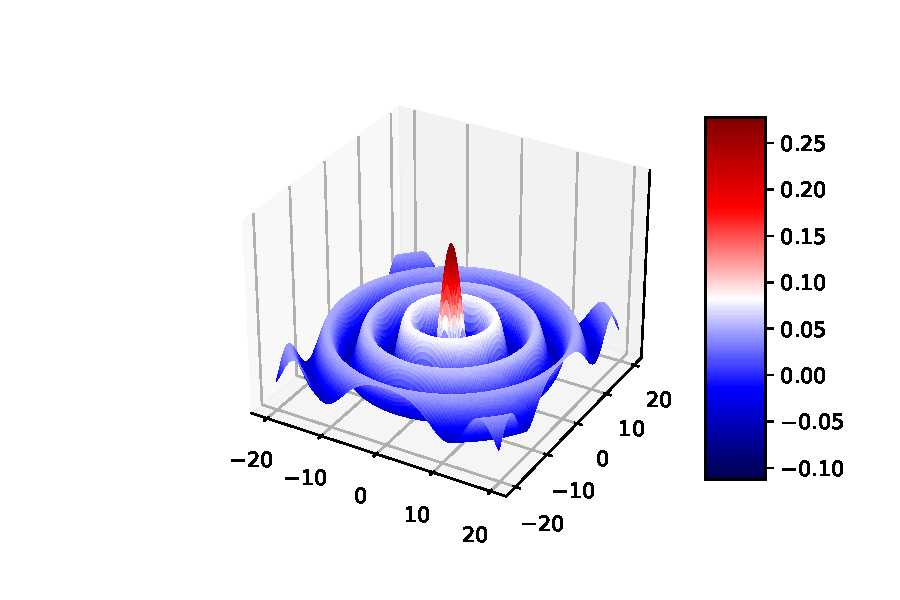
\includegraphics[scale=1]{funcionesbessel0.pdf}
\caption{función de ondas para $l=0,m=0$}
\label{Fig:funcionesbessel0}
\end{figure}


\begin{figure}[h!] \centering
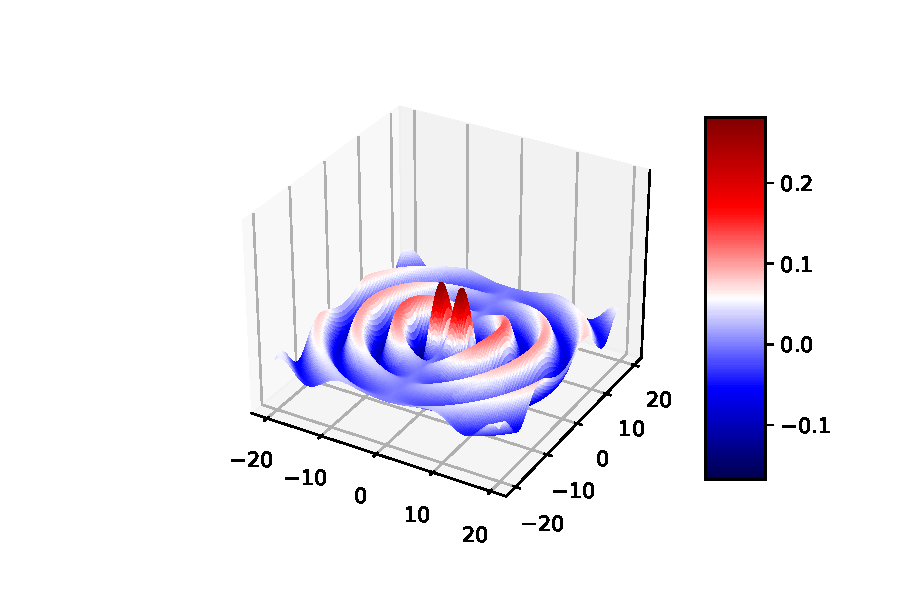
\includegraphics[scale=1]{funcionesbessel1.pdf}
\caption{función de ondas para $l=1,m=0$}
\label{Fig:funcionesbessel1}
\end{figure}

\begin{figure}[h!] \centering
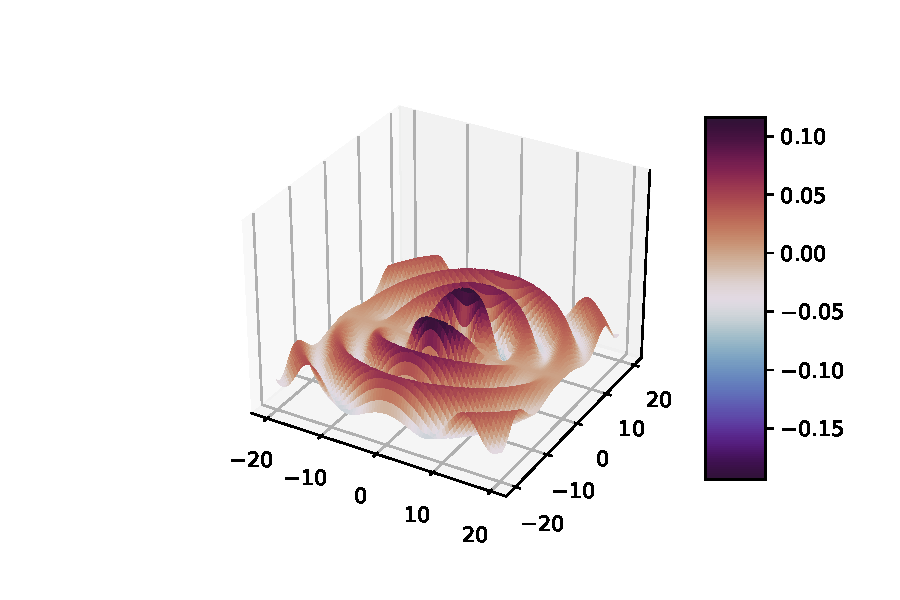
\includegraphics[scale=1]{funcionesbessel1-1.pdf}
\caption{función de ondas para $l=1,m=1$}
\label{Fig:funcionesbessel1-1}
\end{figure}

\begin{figure}[h!] \centering
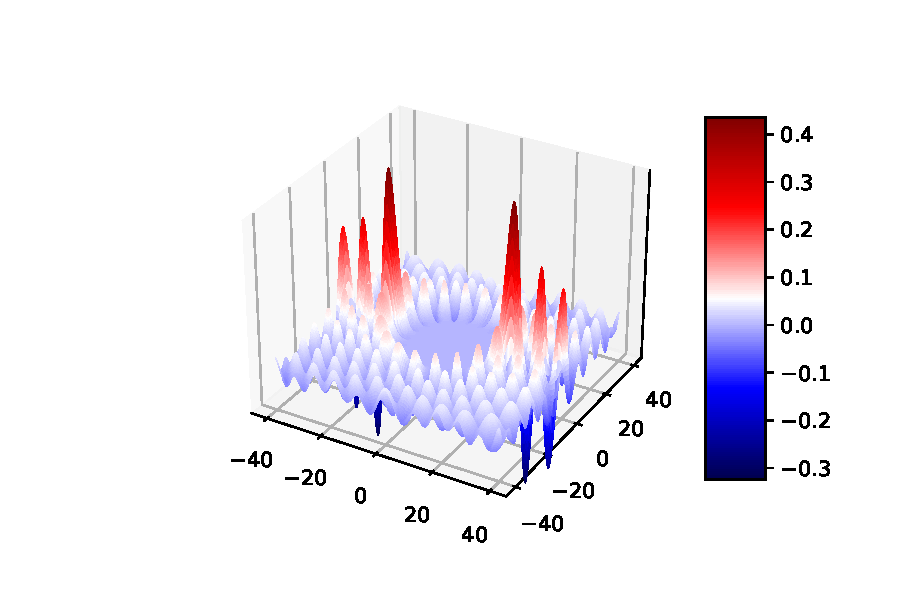
\includegraphics[scale=1]{funcionesbessel20.pdf}
\caption{función de ondas para $l=20,m=0$}
\label{Fig:funcionesbessel20}
\end{figure}

\newpage

\section{Magnetón de Bohr}

Toda partícula con momento angular que posea carga eléctrica adquiere automáticamente un momento magnético $\nmu$. Para un electrón cor carga $-|e|$ y masa $m_e$ que ocupa el punto $\rn$ con momento $\pn = mm_e \vn$, el \textbf{momento magnético} viene dado por:

\begin{equation}
\nmu = \dfrac{1}{2} (\rn \times e \vn) = \parentesis{\dfrac{e}{2 m_e}} \Ln
\end{equation}

Dicha expresión nos dice que el vector momento magnético y el momento angular son proporcionales, paralelos si la carga es positiva y antiparalelos si la carga negativa. Como es bien conocido, un dipolo magnético en presencia de un campo magnético externo $\Bn$ le confiere una energía:

\begin{equation}
E = - \nmu \Bn
\end{equation} 

Supongamos que nuestro campo magnético está definido entorno al eje $z$ tal que $\Bn = B_z \zn$ sin pérdida de generalidad. Entonces solo influirá la componente de $\zn$ del momento angular $L_z$ sobre la energía. Como $L_z$ está cuantizado en múltiplos de $\pm \hbar$, el momento magnético también se va a cuantizar tal que su \textit{quantum}:

\begin{equation}
\mu_B \equiv \dfrac{|e| \hbar}{2 m_e}
\end{equation}
que se llama \textbf{magnetón de Bohr} en la naturaleza. Podemos escribir la siguiente ecuación vectorial para una carga eléctrica:

\begin{equation}
\nmu_l = - \dfrac{\mu_B}{\hbar} \Ln
\end{equation}
tal que el momento magnético $\mu_l$ viene cuantizado por:

\begin{equation}
| \mu_l | = \sqrt{l (l+1)} \nmu_B \quad \mu_{l,z} = - m_l \mu_B
\end{equation}

Consecuencia directa de esto es que la energía de una partícula en presencia de un campo magnético venga cuantizada exactamente igual que el momento angular $L_z$. Surge entonces la obligatoria pregunta: ¿Cuál será el factor giromagnético que corresponde al espín, al giro intrínseco del electrón alrededor de sí mismo? En principio sus valores deben ser exactamente iguales que los del momento angular normal, tal que:

\begin{equation}
|\Sn| = \sqrt{s(s+1)} \hbar \tquad S_z = m_s \hbar 
\end{equation}
\begin{equation}
\nmu_s = g_s \dfrac{\mu_Q}{\hbar} \Sn  \tquad | \nmu_s | = g_s \sqrt{s(s+1)} \mu_Q \tquad \mu_{s,z} = g_s m_s \mu_Q
\end{equation}

donde $\mu_Q$ es el \textit{magnetón de electrón} si nos referimos al espín del electrón o el \textit{magnetón nuclear} $\mu_N \equiv |e| \hbar / (2 m_p)$  para el caso del protón y neutrón. El factor $g_s$ se llama factor giromagnético, y debe ser evaluado experimentalmente para cada partícula. \\

Habiendo asociado la energía con el el momento angular asociar el \textit{operador Hamiltoniano} $H_L$ y $H_S$ con el operador momento angular y el campo $\Bn$. Este Hamiltoniano puede usarse como parte de la ecuación de Schrödinger para obtener la evolución en el tiempo de la función de ondas bajo un campo magnético externo. \\

La influencia de un campo magnético sobre un electrón fue estudiado por Pieter Zeeman. Pensemos que la energía del electrón está cuantizada en niveles $n=1,2,3...$; pero si aparece un término en el hamiltoniano mas allá del potencial de Coulomb entre partículas como es $H_L$ o $H_S$ aparecerá un \textit{desdoblamiento} de las energías de los electrones. Pieter Zeeman encontró este efecto estudiando la frecuencia de los fotones emitidos cuando un electrón caía de un estado mas excitado a otro, en presencia o no de un campo magnético. 

\section{Estados de Polarización Lineal}

Como hemos visto en el tema del momento angular la dependencia de la función de onda es $e^{i \phi}$. Lo visto en el propagador de Feynman permite a ese cuerpo girar simultáneamente en sentidos opuestos alrededor del eje $Z$, ya que \textit{recorre todos los caminos posibles}, como ya hemos visto. Esto aplica tanto al comportamiento respecto el tiempo, ya que sabemos que $\Psi \varpropto e^{-i \dfrac{H}{\hbar} t}$; y al comportamiento respecto el ángulo $\Psi \varpropto e^{- i m_l \phi}$ . Como sabemos existe una identidad entre números complejos:

\begin{equation}
\dfrac{1}{2} \parentesis{e^{i \phi }  + e^{i \alpha} e^{- i \phi}} = \cos \parentesis{\phi - \frac{\alpha}{2}} e^{i \alpha/2}
\end{equation}
donde $\alpha$ es un desfase angular cualquiera $\alpha \in [0,2 \pi]$. Por ser números complejos cualquier combinación lineal puede implicar la suma de un desfase complejo, siempre que se cumpla la propiedad de normalización. Si estudiamos el caso de una suma lineal de estados $m_l=1,-1$ para el ángulo $\Phi$ de tal modo que podemos definir un \textit{estado de polarización lineal} como:

\begin{equation}
| \Psi_{alha} \rangle \equiv | \mathrm{lin}, \alpha/2 \rangle \equiv \dfrac{1}{\sqrt{2}} |1,1\rangle + \dfrac{e^{i \alpha}}{\sqrt{2}} |1,- 1 \rangle\equiv \dfrac{1}{\sqrt{2}} |1\rangle + \dfrac{e^{i \alpha}}{\sqrt{2}} | - 1 \rangle
\end{equation} 
de tal modo que, considerando los armónicos esféricos definidos, la función de ondas angular puede venir dada por:

\begin{equation}
\Psi_{\alpha} (\theta,\phi) = - i \sqrt{\frac{3}{4 \pi}} \sin \theta \sin (\phi - \alpha/2) e^{+ i \alpha/2}
\end{equation}
donde su parte radial no la hemos determinado. Supongamos que tenemos un campo magnético orientado hacia el eje $z$. La energía, si no tiene ningún tipo de potencial externo afectado, vendrá dada únicamente por la relación $E = - \nmu \Bn$, de tal modo que está \textit{cuantizada}, de tal manera que $E_1 = \nmu_B \Bn, E_2 = - \nmu_B \Bn$, y por tanto la frecuencia $\omega_{1,2} = \pm \nmu_B \Bn / \hbar$ de tal modo si $\omega_L = \nmu_B \Bn / \hbar$ podemos expresar la evolución temporal de Schrödinger:

\begin{equation}
| \Psi_{\alpha} (t) \rangle = \dfrac{e^{-i \omega_1 t}}{\sqrt{2}} \parentesis{ | + 1 \rangle + e^{i (\alpha_0 + 2 \omega_L t)} | - 1\rangle}
\end{equation}
donde el $\alpha_0$ es el desfase proveniente del ángulo azimutal. Esta ecuación tiene un claro significado: el dipolo magnético precesa alrededor el campo magnético, dando lugar al conocido fenómeno  de la \textbf{precesión de Larmor}. \\

Además el estado de polarización lineal permite interpretar de manera cuántica el giro dextrógiro y levógiro de las ondas circularmente polarizadas. Como el campo magnético y eléctrico giran en dicha a derechas o izquierdas, es obvio que el fotón debe contener esa información, en este caso en el \textit{espín}. Por tanto un quantum de energía lleva energía, momento y momento angular. \\

El valor para el espín de un fotón que se propaga en la dirección $z$ es $S_z = \pm \hbar$ (valores experimentales). Eso sugiere que el módulo del espín es $1$. Uno podría pensar que $0$ también debería ser un estado posible (el fotón no lleva momento angular en la dirección de propagación). Esto es imposible debido al carácter relativista del fotón (propagándose a la velocidad de la luz). Si el momento angular $L$ tuviera algún tipo de componente en el eje $x$ o $y$ significaría que los campos electromagnéticos rotarían en la dirección de propagación, teniendo una componente longitudinal. \\

Esto significaría que los campos se irían moviendo hacia delante y atrás, que es incompatible con la relatividad por la \textit{contracción de Lorentz}. Es evidente que la contracción de Lorentz hace que no exista componente $z$ para el fotón, y por tanto no pueda existir una oscilación en dicha dirección. 


\section{El átomo de hidrógeno}

El átomo de hidrógeno es el átomo mas sencillo de todos, constando de un protón en el núcleo y un electrón orbitando entorno a este. Otros átomos presentan combinaciones mucho mas complicadas en las que la energía potencial de un electrón viene dada por la atracción de un núcleo y la repulsión de los otros electrones (entre otros muchísimos factores) haciendo muy complicado su estudio. Esto sin embargo no debe consternar al lector: escribiremos un caso general para $Z$ protones. ¿Por qué? Porque los electrones mas cerca del núcleo según la ley de Gauss solo se verán afectados por las cargas del núcleo. \\

Sin embargo en este átomo de Hidrógeno podemos suponer que solo hay un potencial, el potencial de Coulomb:

\begin{equation}
U(r) = \dfrac{- Z e^2}{4 \pi \varepsilon_0} \dfrac{1}{r}
\end{equation}

Por ser un potencial de simetría central podemos buscar soluciones de la ecuación $H \Psi = E \Psi$  en coordenadas esféricas, tal que:

\begin{equation}
\Psi (r, \theta, \phi ) = R_l(r) Y_l^{m_l} (\theta, \phi)
\end{equation}

Para que tenga solución el problema se debe verificar que la energía debe venir dada por la siguiente ecuación:

\begin{equation}
E_n = \dfrac{-1}{(4 \pi \varepsilon_0)^2} \dfrac{m Z^2 e^4}{2 \hbar^2} \dfrac{1}{n^2} \quad n = l+1, l+2,...
\end{equation}
que básicamente nos da los posibles valores de energía que puede tener el sistema para un momento angular dado. Sin embargo solemos expresar el posible momento angular para un estado de energía dado, de tal forma que: $n=1,2,3...$ y $l=0,1,...,n-1$. Dado que cada valor de $l$ arrastra consigo una degeneración de energía (i. e. para la misma energía (autovalor de la energía) existen varias funciones de onda (autofunciones)) de tal manera que para un nivel $n$ de energía su \textit{degeneración} es:

\begin{equation}
g_n = \sum_{l=0}^{n-1} (2l+1) = n^2
\end{equation}

este fenómeno de que para un mismo estado de energía contemplemos diferentes funciones de ondas solo ocurre con los potenciales proporcionales $1/r$ y $r^2$. Cualquier otro potencial $U(r)$ hubiera generado energías $E_{nl}$ dependientes de los índices $n$ y $l$. El resultado final, para las funciones que definen los estados $| E_n l m-l \rangle$ para el hidrógeno es:

\begin{equation}
\Psi_{n l m_l} = N_{nl} e^{- Z r / (n a_0)} L^{2l+1}_{n-l-1} (\rho) \rho^{l} Y_l^{m_l} (\theta, \phi)
\end{equation}
donde $N_{lm}$ es el factor de normalización, $a_0$ es el radio de Bohr (radio mas probable para el electrón caso Z=1). Definimos estos términos y $\rho$ como:

\begin{equation}
N_{nl} = \ccorchetes{\parentesis{\dfrac{2Z}{n a_0}}^3\dfrac{(n-l-1)!}{2n (n+l)!}}^{1/2} \quad a_0 \equiv \dfrac{4 \pi \varepsilon_0 \hbar}{m e^2} \quad \rho \equiv \dfrac{2 Z r}{n a_0}
\end{equation}
Además $L(\rho)$ no es otro que los polinomios de Laguerre definidos como:

\begin{equation}
 L_q (x) \equiv \dfrac{1}{q!} e^x \parentesis{\derivadas{}{x}}^q (e^{-x} x^q ) \equiv \sum_{k=0}^{q} (-1)^k  \binom{q}{k} \dfrac{1}{k!} x^k
\end{equation}
\begin{equation}
L_{q-p}^{p} \equiv (-1)^p \parentesis{\derivadas{}{x}}^p L_q(x) 
\end{equation}
El conjunto de autofunciones $\Psi_{n l m_l} (\rn ) \equiv | n l m_l \rangle$ del átomo de hidrógeno constituyen una base ortonormal dentro del subestapcio de Hilbert de $L^2$ formado por los estados de energía $E<0$.

\section{El espín del electrón}

El espín del electrón es uno de los casos mas misteriosos de la física cuántica, ya que pone en entre dicho uno los postulados mas importantes de esta: el carácter univaluado de la función de ondas. Como ya hemos dicho esperamos del espín un comportamiento similar al de el momento magnético, tal que venga cuantizada por multiplos enteros de $\hbar$. Sin embargo el experimento de Stern-Gerlach, que mas adelante describiremos, no solo demostró que esto era categóricamente falso, si no que además es el factor es $\pm 1/2$, tal que:

\begin{equation}
S_z = \pm \hbar / 2 \tquad m_s = -1/2, 1/2
\end{equation}
mientras que el factor giromagnético es

\begin{equation}
g_e = -2
\end{equation}
de tal manera que el momento dipolar magnético continúa siendo proporcional al magnetón de Bohr. \\

Como sabemos $ \Psi (\phi) \varpropto e^{i m_s \phi}$, por lo que definimos el intervalo del ángulo por $\phi \in [0,2\pi]$ vemos que la función de ondas es \textit{multievaluada}, ya que $\Psi(0) = - \Psi (2 \pi)$, dando lugar a que \textit{tras una rotación de 360º el estado del electrón cambia de signo}. No es multivaluada la función $|\Psi|^2$. Dicho carácter tumbaría toda la física cuántica vista hasta el momento, por lo que lo que se hizo fue aumentar el intervalo en el que vive el ángulo $\phi$, tal que  $\phi \in [0,4 \pi]$.  De este modo que ahora sí sería univaluada. \\ 

La interpretación de los valores $s=1/2$ y $g_e = -2$ fue realizada por Dirac, descrita como una consecuencia de la ecuación relativista para el movimiento libre del electrón (ecuación de Dirac), que describe la propagación hacia atrás en el tiempo en forma de antipartícula. \\

Habiendo demostrado que existen \textbf{dos} estados cuánticos independientes, queda fijada la dimensión del espacio de Hilbert en que deben residir todos sus estados cuánticos (2). Como sabemos un espacio de Hilbert es un espacio donde habitan las posibles funciones de ondas de nuestro problema, pudiendo expresarse como la combinación lineal de autofunciones linealmente independientes. Como solo existen dos autovalores posibles solo existirán dos autofunciones, y por tanto podremos escribir cualquier estado como combinación lineal de estos. Es común describir los estados base del espacio de dimensión 2 matricialmente:

\begin{equation}
\eup \equiv \begin{pmatrix}
1 \\
0
\end{pmatrix} \tquad \edw \equiv \begin{pmatrix}
0 \\
1
\end{pmatrix}
\end{equation}
Consecuentemente el estado de espín mas general del electrón puede escribirse como:
\begin{equation}
| \chi \rangle = c_1 \eup + c_2 \edw \tquad | c_1 |^2 + |c_2 |^2 = 1; \quad c_1, c_2 \in \mathbb{C}
\end{equation}
tal que podemos definir con un solo parámetro haciendo $c_1 = \cos (\theta/2)$ y $c_2 = \sin ( \theta / 2)$ tal que $\theta \in [0,\pi]$. Podemos interpretar entones podemos interpretar, si existe un desfase complejo completamente válido, donde $\phi \in [0,2\pi]$, tenemos que:

\begin{equation}
| \chi \rangle = \cos (\theta/2) \eup + e^{i \phi} \sin(\theta/2) c_2 \edw 
\end{equation}

Ahora tenemos que conocer cual es la dimensión y forma de los operadores espín, $S_x,S_y,S_z$ en este espacio de Hilbert. Aunque no lo hayamos visto, podemos expresar cualquier operador de manera matricial, una forma completamente análoga a la diferencial. Por ejemplo vamos a expresar el operador $L_z$ para $l=1$ en forma matricial: \\


\shadowbox{\textbf{Ejemplo 15.1}}

\hrulefill

Como sabemos $L_z$ viene dada, en forma diferencial, tal que $L_z = - \hbar \parciales{}{\phi}$. Entonces como estamos intentando calcular la forma matricial cuando $l=1$, el espacio de Hilbert para la función de ondas angular $Y_l^{m_l}$ es de dimensión 3, tal que podemos expresarlo de manera matricial. En ese caso está claro que

\begin{equation}
Y_1^1 = \begin{pmatrix}
1 \\ 0 \\ 0
\end{pmatrix}
\tquad Y_1^0 = \begin{pmatrix}
0 \\ 1 \\ 0
\end{pmatrix}
\tquad Y_1^{-1} = \begin{pmatrix}
0 \\ 0 \\ 1
\end{pmatrix} 
\end{equation}
Ahora tenemos que estudiar como actúa el operador para dichas funciones, tal que:

$$L_z Y_1^1 =  - \hbar Y_1^1 \tquad L_z Y_1^0 = 0 \tquad L_z Y_1^{-1} = \hbar Y_1^{-1}$$
por lo que expresado de manera matricial queda claro que:

\begin{equation}
L_z = \hbar \begin{pmatrix}
-1 & 0 & 0 \\
0 & 0 & 0 \\
0 & 0 & 1
\end{pmatrix}
\end{equation}

Podemos hacer exactamente lo mismo para $L_x$ y $L_y$ de manera análoga

\hrulefill \\

Como podemos ver podemos expresar \textit{cualquier operador} de manera matricial, por lo que los operadores espín no serán diferentes. Ahora bien ¿Cuál es su forma matricial? Si suponemos que el espín representa un giro instantáneo (aunque en realidad no sabemos exactamente lo que es) sabemos que deben verificar entre si las mismas propiedades que verifica cualquier giro instantáneo, que es básicamente una relación de conmutación. La relación de conmutación nos dice que:

\begin{equation}
[S_x,S_z] = i \hbar S_z \tquad [S_z,S_x] = i \hbar S_y \tquad [S_y,S_z] = i \hbar S_x
\end{equation} 
¿Que significa exactamente decir que ``deben verificarse las relaciones de conmutación''? Basicamente nos dice que:

\begin{equation}
[S_x,S_y] = S_x \cdot S_y - S_y \cdot S_x = i \hbar S_z
\end{equation}
ya que $S_x \cdot S_y \neq S_y S_x$. Esto es una propiedad de todo giro intrínseco, verificándose de igual manera para $L$. De hecho esto se deriva del estudio de las propiedades del rotacional, ya que si $\Rn \equiv \rn \times \nabla$, podemos comprobar que $[R_x,R_y] =  - R_z$, ya que \textit{las propiedades geométricas} de las rotaciones espaciales deben ser trasladadas a la física cuántica. Entonces puede comprobarse fácilmente que:

\begin{equation}
S_x =  \dfrac{\hbar}{2} \sigma_1 \tquad S_y = \dfrac{\hbar}{2} \sigma_2 \tquad S_z =\dfrac{\hbar}{2} \sigma_3
\end{equation}
de tal modo que:
\begin{equation}
\sigma_1 \equiv \begin{pmatrix}
0 & 1 \\
1 & 0 
\end{pmatrix}
\tquad 
\sigma_2 \equiv \begin{pmatrix}
0 & -i \\
i & 0 
\end{pmatrix} \tquad
\sigma_3 \equiv \begin{pmatrix}
1 &  0  \\
0 & -1 
\end{pmatrix}
\end{equation}
conocidas en la literatura como \textbf{matrices de Pauli}. Será coser y cantar demostrar que los ángulos $\theta$ y $\phi$ que antes hemos usado como meros coeficientes para describir el estado cuántico mas general para el espín de un \textit{fermión} (electrón, neutrón, protón...) corresponden en la realidad al ángulo a donde apunta el promedio temporal del espín $\langle \Sn \rangle_{\chi}$. A la esfera en la cual debe vivir nuestro espín promedio se le llama \textbf{esfera de Bloch}, donde los ángulos $(\theta,\phi)$ nos definen hacia donde apunta dicho promedio. Calculemos entonces el promedio de $\Sn$ t:

\begin{equation}
\langle \Sn \rangle = \langle \chi | \Sn | \chi \rangle \rangle = \begin{pmatrix}
\langle \chi | S_x | \chi \rangle \\ \\
\langle \chi | S_y | \chi \rangle \\ \\
\langle \chi | S_z | \chi \rangle 
\end{pmatrix}
\end{equation}
de tal modo que ser verificará sin lugar a dudas que:

\begin{equation}
\langle \chi | S_x | \chi \rangle = \frac{\hbar}{2}
\begin{pmatrix}
\cos \theta/2 \\
 e^{-i\phi} \sin \theta/2
\end{pmatrix}^T \begin{pmatrix}
0 & 1 \\
1 & 0 
\end{pmatrix}
\begin{pmatrix}
\cos \theta/2 \\
 e^{-i\phi} \sin \theta/2
\end{pmatrix} = \frac{\hbar}{2}  \sin \theta \cos \phi
\end{equation}
\begin{equation}
\langle \chi | S_y | \chi \rangle = \frac{\hbar}{2}
\begin{pmatrix}
\cos \theta/2 \\
 e^{-i\phi} \sin \theta/2
\end{pmatrix}^T \begin{pmatrix}
0 & -i \\
i & 0 
\end{pmatrix}
\begin{pmatrix}
\cos \theta/2 \\
 e^{-i\phi} \sin \theta/2
\end{pmatrix} = \frac{\hbar}{2}  \sin \theta \sin \phi
\end{equation}
\begin{equation}
\langle \chi | S_z | \chi \rangle = \frac{\hbar}{2}
\begin{pmatrix}
\cos \theta/2 \\
 e^{-i\phi} \sin \theta/2
\end{pmatrix}^T \begin{pmatrix}
1 & 0 \\
0 & -1 
\end{pmatrix}
\begin{pmatrix}
\cos \theta/2 \\
 e^{-i\phi} \sin \theta/2
\end{pmatrix} = \frac{\hbar}{2}  \cos \theta 
\end{equation}
de tal forma que:

\begin{equation}
\langle \Sn \rangle = \dfrac{\hbar}{2} \begin{pmatrix}
\sin \theta \cos \phi \\
\sin \theta \sin \phi \\
\cos \theta
\end{pmatrix}
\end{equation}
como ya hemos mencionado. También resulta interesante estudiar como se comporta el espín bajo la acción de un campo magnético (como varía temporalmente), tal y como pasa con el experimento de Stern-Gerlach. Supongamos que tenemos un campo magnético orientado hacia el eje $z$. Entonces la energía vendrá dada por:

\begin{equation}
E = \nmu \cdot \Bn = g_s \dfrac{\mu_Q
 B}{\hbar} S_z = g_s \dfrac{\mu_Q B}{\hbar} \dfrac{\hbar}{2}  \begin{pmatrix}
 1 & 0 \\
 0 & -1 
 \end{pmatrix}
\end{equation}
donde $g_s$ es el \textit{factor giromagnético} y $\mu_Q$ es el magnetón correspondiente (magnetón de Bohr si estudiamos un electrón, magnetón nuclear si estudiamos un protón o neutrón...). Como sabemos el factor temporal vendrá dado por $e^{-i \frac{H}{\hbar} t}$, por lo que la evolución temporal contendrá una matriz en un exponente. Lidiar con esto no es difícil aunque puede ser una sorpresa para algunos. Llamando $E_0=g_s \mu_Q B$ la función temporal vendrá dada por:

\begin{equation} \mathcal{U} (t) = e^{- i \frac{E}{\hbar} t} = \begin{pmatrix}
\exp(- i \frac{E_0}{2\hbar} t ) & 0 \\
0 &  \exp (i \frac{E_0}{2\hbar} t)
\end{pmatrix} \end{equation}
de tal forma que la función de ondas $\chi (t)$ se podrá expresar como el producto 

\begin{equation}
\chi (t) = \mathcal{U} \cdot \chi_0
\end{equation}

\section{El principio de exclusión de Pauli}

La mecánica cuántica debe describir correctamente no únicamente el movimiento de partículas individuales de masa $m$, sino también el de \textit{conjuntos} de partículas idénticas. Supongamos dos partículas idénticas (por ejemplo dos electrones) ocupando las posiciones $\rn_1$ y $\rn_2$, con dos estados cuánticos diferentes $\Psi_a$ y $\Psi_b$. Como ambos electrones son idénticos pueden ocupar zonas del espacio simultáneamente, vamos a calcular la probabildad de que se disparen simultáneamente dos detectores situados en los puntos $\rn_1$ y $\rn_2$. \\
    
Entonces la función de ondas que gobierne dicha probabildad que debe ser extendida a un espacio de $\mathbb{R}^6$ tal que $\Psi (\rn_1, \rn_2)$. Como las partículas son idénticas (no podemos distinguirlas) es obligatorio admitir que $| \Psi (\rn_1,\rn_2) |^2 = | \Psi (\rn_2,\rn_1) |$. Tenemos que el producto $\Psi = \Psi_a (\rn_1) \Psi_b (\rn_2)$ no puede ser una opción ya que $\Psi = \Psi_a (\rn_2) \Psi_b (\rn_1)$ es radicalmente distinta. Entonces uno puede pensar en que la suma de estados tal que:

\begin{equation}
\Psi_S (\rn_1 , \rn_2) \equiv \dfrac{(\Psi_a (\rn_1) \Psi_b (\rn_2)+\Psi_b (\rn_1) \Psi_a (\rn_2))}{\sqrt{2}}
\end{equation}

aunque es inevitable la reflexión de que tomar la diferencia también cumple dicha condición:

\begin{equation}
\Psi_A (\rn_1 , \rn_2) \equiv \dfrac{(\Psi_a (\rn_1) \Psi_b (\rn_2)-\Psi_b (\rn_1) \Psi_a (\rn_2))}{\sqrt{2}}
\end{equation}

A la suma la llamaremos la \textbf{combinación simétrica} ($\Psi_S$) y a la diferencia la llamaremos la  \textbf{combinación antisimétrica} ($\Psi_A$). En el caso antisimétrico se cumple que  
\begin{equation}
\Psi_A (\rn_1,\rn_2)  = - \Psi_A (\rn_2,\rn_1) 
\end{equation} 

Si consideramos dos electrones de un átomo multielectrónico, cuyo Hamiltoniano contiene la energía de repulsión, es fácil de darse cuenta de que las soluciones simétrica y antisimétrica producen \textit{energías sensiblemente distintas}, ya que cuando las partículas están mas próximas entre sí, que es cuando mas energía electroestática de repulsión habrá, la función de ondas antisimétrica se aproxima a cero: $\rn_1 \approx \rn_2$ implica que $| \Psi_a (\rn_1,\rn_2) | \approx 0$. En el caso de la solución simétrica no ocurrirá este fenómeno. \\

Podemos verlo fácilmente si tratamos de calcular analíticamente la energía de repulsión tal que $H_{12} = (e^2 / 4 \pi)$ con $r_{12} \equiv | \rn_1 - \rn_2 |$. Para una integral en 6D tal que $\D \tau = \D \tau_1 \D \tau_2$ tal que $\D \tau_{1,2} \equiv \D^3 \rn_{1,2}$. Simplificando la notación tal que $\Psi (\rn_{1,2}) \equiv \Psi (1,2)$. Entonces el promedio de la energía:

\begin{equation}
\int \Psi_S^* H_{12} \Psi_S  \D \tau = C+K \tquad \int \Psi_A^* H_{12} \Psi_A D \tau = C-K
\end{equation}
donde

\begin{equation}
C = \int |\Psi_a (1)|^2 |\Psi_b (2)|^2 H_{12} \D \tau \tquad 
K = \int (\Psi^*_a (1) \Psi_b(1)) (\Psi^*_b (2) \Psi_a (2)) H_{12} \D \tau  
\end{equation}
La interpretación de ambas integrales es complicada. La primera $C$ es la repulsión electroestática entre los dos estados cuánticos, ya que según la mecánica cuántica la carga del electrón se distribuye como una función continua. Sin embargo la segunda $K$ se denomina \textbf{energía de intercabio}, y no tiene ningún análogo en el mundo clásico. Es simplemente un reflejo de que ambas partículas estén ocupando simultáneamente cada punto $\rn$ del espacio. De hecho se piensa que la mayor parte de la energía de química de las moléculas proviene de este término. \\
 
Volviendo a la situación general: si tenemos dos partículas idénticas en un problema físico concreto, ¿Que función de ondas debemos usar en nuestro Hamiltoniano? La respuesta no nos la puede dar la física cuántica, si no tenemos que estudiar caso por caso. \\

Por ejemplo para el aso específico de un electrón, partícula con espín $1/2$, tenemos que al realizar una rotación de 360º la función de ondas cambia de signo $\Psi \rightarrow - \Psi$. Entonces si el intercambiamos la posición de los electrones por caminos que no se entrecruzan, tendremos que se ha hecho una rotación \textit{mutua} de 360º (180º cada una).  Eso significa que la función de ondas debe cambiar de signo al intercambiar las posiciones de los electrones, y por tanto \textit{debemos elegir únicamente la solución antisimétrica}. \\

Admitir que la función de ondas debe ser siempre antisimétrica tiene una consecuencia inmediata: si los estados cuánticos son iguales $\Psi_A = 0$. En otras palabras: \textit{en un determinado sistema físico, dos electrones no pueden estar nunca en el mismo estado cuántico}. Este es el famosos \textbf{principio de exclusión} de Wolfgang Pauli. \\

Pesemos ahora en los estados cuánticos del espín que pueden tener los electrones. Como sabemos \textit{los estados de espín residen en un espacio de Hilbert (dimensión 2) distinto de sus excitaciones espaciales}. \\

Supongamos un momento que no conocemos el espín del electrón, de tal modo que pueda tener un estado simétrico o antisimétrico. Es claro que ambos electrones tienen espín arriba o abajo a lo largo del eje Z. Los posibles espines que pueden tener son:  $ \vert \uparrow \uparrow \rangle $, $\vert \downarrow \downarrow \rangle$, $\vert \uparrow \downarrow \rangle$ y $\vert \downarrow \uparrow \rangle$, o una combinación lineal de estos. Sin embargo estos estados no son ortogonales entre sí, por lo que debemos encontrar una serie de 4 estados que sí sean ortogonales entre sí y que conformen nuestro espacio de Hilbert e dimensión 4. \\

 Cuando los espines tienen espín arriba o abajo están en un estado simétrico de espín, de tal forma que $\chi (\rn_1,\rn_2) = \chi (\rn_2,\rn_1)$. Cuando sus espines son opuestos se presentan dos estados matemáticamente distinos:

\begin{equation}
\chi_T = \frac{1}{\sqrt{2}} ( \vert \uparrow \downarrow \rangle + \vert \downarrow \uparrow \rangle) \tquad \chi_0 = \frac{1}{\sqrt{2}} ( \vert \uparrow \downarrow \rangle - \vert \downarrow \uparrow \rangle)
\end{equation}
que se llaman los \textbf{estados triplete} ($\chi_T$) y \textbf{singlete} ($\chi_0$). Entonces los posibles estados de electrones posibles (estados ortogonales entre sí) son 4, que son el singlete, el triplete además de $| \uparrow \uparrow \rangle$ y $| \downarrow \downarrow \rangle$. Se puede comprobar la ortogonalidad definiendo el producto escalar de dicho espacio como:

\begin{equation}
  \langle \alpha_1 \beta_1 \vert \alpha_2 \beta_2 \rangle = \langle \alpha_1 \vert \alpha_2 \rangle \cdot \langle \beta_1 \vert \beta_2 \rangle
\end{equation}
todos los estados son simétricos a excepción del estado singlete. Esto es sumamente importante, ya que es esta característica la que permite que exista el \textit{principio de máxima multiplicidad de Hund}. 

Debemos resaltar que el \textit{carácter antisimétrico} de la función de ondas para el electrón no implica que la función de ondas espín sea antisimétrica, implica que la \textit{función de ondas global} (que es el producto de la función de ondas espacial y la función de ondas espín) es antisimétrica. Si es $\Psi=\psi \chi$ tenemos que las únicas combinaciones posibles son:

\begin{equation}
\Psi = \psi_S \chi_A \tquad \Psi = \psi_A \chi_S
\end{equation}

Tenemos varios ejemplos para cada caso. Por ejemplo si tenemos dos electrones orbitando una capa $p$ como pueden ser los dos últimos electrones del oxígeno, dichos electrones debido a las fuerzas de repulsión electroestáticas (además de las fuerzas dipolares o magnéticas) tratarán de encontrarse lo mas alejadas posibles. En este caso se encontrarán en estados ortogonales como puede ser en $2p_x$ o $2p_y$, de tal modo que la energía se minimiza. Obviamente la función de ondas espacial en este caso será antisimétrica, por lo que no queda otra (para mantener la función de ondas antisimétrica) que la función de ondas espín sea simétrica, y por tanto que ambos espines estén orientados hacia la misma dirección (también podrían estar en estado triplete, aunque generalmente no ocurre, sobretodo en casos con 3 electrones). Es esta la explicación a la \textbf{regla de Hund}. \\

El caso inverso ocurre por ejemplo con el Helio. Los dos electrones que poseen son del tipo $1s$ por lo que por tener funciones de ondas espaciales simétricas deben tener funciones de ondas de espín antisimétricas, y por tanto un estado singlete; dejando así la función de ondas general en un estado antisimétrico.\\

La antisimetría y simetría es un fenómeno mucho mas trascendenta. Estudiamos el caso para los electrones, pero en realidad tiene un papel tan fundamental que divide por completo la materia en dos tipos: los \textbf{fermiones} y los \textbf{bosones}. \\

Los fermiones son los electrones, quarks, protones... y son aquellos elementos que tienen un espín semientero y por tanto una función de ondas antisimétrica. \\

Los bosones son los fotones, gluones, fononoes...  y tienen un espín entero, por tanto una función de ondas simétrica. Esto lleva a fenómenos como el láser, que es un haz de fotones muy denso los cuales tienen el mismo estado. Dicho fenómeno jamas podría ocurrir con los electrones. 


\section{Partícula encerrada en un Cubo \label{Sec:24}}

Vamos a analizar (usando la ec. de Schrödinger) el caso de una partícula (electrón, fotón...) encerrada entre 6 paredes impenetrables situadas a una distancia $L$. Es decir, nuestra partícula estará encerrada en un cubo de lado $L$. Primero resolveremos el problema en 1D (para uno de los lados) para luego generalizar al caso 3D. En dicho cubo no existe ningún tipo de energía potencial; la única condición impuesta es que la particula no salga de dicho cubo. Para esto podemos suponer que fuera del cubo el potencial es infinito $U(0)=U(L) = \infty$ ya que ninguna partícula puede vivir en un potencial infinito. La ec. de Schrödinger para potencial nulo tiene que $\hbar^2 \partial^2 \Psi / \partial x^2 = 2 m E \Psi (x)$, tal que su solución general es: 

\begin{equation}
\Psi (x) = A e^{-ikx} + B e^{ikx}
\end{equation}
con $k = \sqrt{2mE}/\hbar > 0 $. Las condiciones de contorno son: $\Psi(0) = \Psi(L) = 0$ de tal modo que se debe verificar:

\begin{equation}
A =  - B \tquad k_n L = n \pi
\end{equation}
Normalizando las soluciones para los estados normalizados tendremos que:
\begin{equation}
\Psi_n (x) = C_n \sin (k_n x) \tquad C_n = \sqrt{\frac{2}{L}}
\end{equation}
Como $k_n = \frac{n \pi}{L}$ tendremos que las energías permitidas para la partícula \textit{están cuantizadas} de tal modo que:

\begin{equation}
E_n = \frac{\hbar^2 \pi^2}{2m L^2} n^2
\end{equation}
siendo compatible con dos hechos ya conocidos: cuando $n \rightarrow \infty$ la diferencia relativa de energías es menor convirtiéndose el espectro de energías en un espectro continuo (si $n \gg \infty$) y que cuando $L\rightarrow 0$ la energía tiende a infinito, ta y como nos dice el \textit{prinicipio de indeterminación}. Para el caso de un fotón:

\begin{equation}
E_n = \frac{\pi \hbar c}{L} n
\end{equation}

De hecho que la \textit{energía} esté cuantizada es una consecuencia de que el \textit{momento} esté cuantizado ($|p_n| = n \pi \hbar /L$ tal que $E = \sqrt{p^2 c^2 + m^2 c^4}$ para el caso ultrarrelativista o $E = p^2 /2m$ para el caso no relativista). Es completamente análogo decir que la longitud de onda posible esté cuantizada, dada la relación de De Broglie entre $p$ y $\lambda$. La extensión a 3D resulta sencilla:

\begin{equation}
\Psi_{n_1,n_2,n_3} = \parentesis{\dfrac{2}{L}}^{3/2} \sin \parentesis{\frac{n_1 \pi x}{L}}\sin \parentesis{\frac{n_2 \pi y}{L}} \sin \parentesis{\frac{n_3 \pi z}{L}}
\end{equation}
con energías:

\begin{equation}
E_{n_1,n_2,n_3} = \frac{\hbar^2 \pi^2}{2m L^2} \parentesis{n_1^2+n_2^2+n_3^2}
\end{equation}
Somos capaces ahora de darle un mayor significado físico a la degeneración cuántica o degeneración de la energía. Para una misma energía existen diferentes patrones de $n_1,n_2,n_3$ (\textit{ternas}) que cuantifican esa energía. Ahora bien, ¿Cómo calculamos cuantos estados hay en un intervalo de momentos/energía? Si $n_i \rightarrow \infty$ (\textit{límite clásico}) y suponemos un \textit{intervalo continuo} de energías/momentos; podemos suponer que en el espacio de momentos (figura ) un elemento en un elemento diferencial de volumen $\D \pn^3$ contiene un número de estados determinado. Dado que $$ p_n = n h / 2 L $$ tendríamos que $ \D N  = \D^3 \pn / ( h/2L)^3 $. Sin embargo hay un error en esta formula: no estamos teniendo en cuenta que tenemos dos signos posibles del momento en cada eje $p_n = 2 n h /2 L = n h /L$. La fórmula final vendrá dada entones por:

\begin{equation}
\D N = \dfrac{\D^3 \pn}{(h /L)^3}; \tquad \dfrac{\D N}{V} = \dfrac{\D^3 \pn}{\hbar}
\end{equation}
esta ecuación es completamente relativista, aunque para relacionar el número de estados cuánticos y la energía usamos una aproximación no relativista tal que $E=p^2/2m$. En ese caso $\D p = \sqrt{\frac{2 m}{ E}} \D E$. No obstante hemos usado $\D^3 \pn$, no $\D p$. Asi que tendremos que relacionar $\D \pn$ con $\D p$ de alguna forma. La mejor forma para relacionar esto es usar las coordenadas esféricas de tal modo que $\D^3 \pn = p^2 \D p \D \Omega$ tal que sobre un ángulo sólido $\int \D \Omega = 4 \pi$. En ese caso podemos relacionar directamente:

\begin{equation}
\D N = \dfrac{4 \pi V}{h^3} p^2 \D p
\end{equation}
o en función de la energía:

\begin{equation}
\D N = g(E) \D E = \dfrac{4 \pi V}{h^3} \parentesis{2 m^3}^{1/2} E^{1/2} \D E
\end{equation}
donde $g(E)$ no es otra cosa que la \textbf{degeneración cuántica} para cierto estado de la energía. En realidad $\D N$ es un número entero ya que es el número de estados que una molécula puede ocupar fijado el valor de la energía; donde $g(E)$ puede interpretarse como la densidad de estados cuánticos. Dicha densidad es la contribución de cada partícula a la entropía del sistema. \\

De hecho ya fue Boltzmann el que definió la entropía como $S = k_B \ln W$. Aunque este le dio una interpretación incorrecta a dicho parámetro, hoy en día asociamos $W$ al número de estados cuánticos que puede tener un gas de $N$ moléculas encerradas en el volumen $V$. Dicho número es claro: se trata de multiplicar la degeneración de cada nivel de energía por todos los niveles elevada al número de moléculas que se encuentran en ese nivel teniendo en cuerta que todas las moléculas son idénticas y por tanto no podemos contar como estados cuánticos distintos sus distintas permutaciones. En ese caso: $W = \prod_i (g_i^{n_i} /(n_i)!)$.  


% Escribir las expresiones cuando las longitudesno son iguales y caso fotón con mas fuerza

\section{El salto de potencial}

A continuación vamos a estudiar como se comporta la función de ondas unidimensional cuando existe una región con un potencial nulo y otra con un potencial constante $E_0>0$. El estudio de este tema es muy importante ya que es la antesala al \textit{efecto túnel}, uno de los fenómenos cuánticos mas importantes. \\


Supongamos entonces que se verifica que $U=0$ si $x<0$ y que $U=E_0$ si $x \geq 0$, de tal modo que existe un escalón donde la fuerza, teóricamente, sería infinita. En la realidad $F=- \partial U / \partial x$ nunca será infinita, de tal forma que nunca tendrá una forma de escalón si tenemos una resolución lo suficientemente alta. De todas maneras esto no nos importa, nosotros asumiremos que esta descripción es válida. \\

Resolvemos la ecuación de Schrödinger buscando los estados estacionarios. En todos estos problemas aparecerán funciones del tipo $Ae^{\pm ik  x}$ (ondas planas). Como ya sabemos se tratan de \textit{funciones ideales} que no son de cuadrado sumable, por lo que tenemos que darle una interpretación plausible al coeficiente $A$. \\

El módulo de $A$ se asociará al \textit{flujo de partículas por unidad de tiempo} $\phi$ que circulan por un punto $x$ con velocidad $v$ tal que $\phi = v |A|^2$ . La fase de $A$ tiene sentido cuando se encuentra en combinación lineal con otras, codificando justamente el desfajase entre estas. \\

Para estudiar lo que ocurre con la partícula resolvemos la ecuación de Schrödinger para los estados estacionarios suponiendo que la partícula incide desde el lado izquierdo. Aunque podamos parametrizar el pulso incidente resolviendo la ecuación temporal, obteniendo una solución mucho mas realista, nos interesa el caso en el que la energía es perfectamente conocida $\Delta E \rightarrow 0$ de tal modo que no nos importa el tiempo $\Delta t \rightarrow \infty$. \\

Designamos como $\Psi_1$ la función de ondas en el lado izquierdo y $\Psi_2$ ene lado derecho, de tal modo que existe una onda incidente y reflejada que vive en el lado izquierdo y una trasmitida en el lado derecho, tal que:

\begin{equation}
\Psi_1 = A e^{ik_1x} + B e^{-ik_1 x} \tquad \Psi_2 = C e^{ik_2x} \tquad A,B,C \in \mathbb{C}
\end{equation}
donde claramente los coeficientes dependerán del nivel de energía, tal que:

\begin{equation}
k_1 \equiv \dfrac{\sqrt{2mE}}{\hbar} \tquad k_2 \equiv \dfrac{\sqrt{2m(E-E_0)}}{\hbar}
\end{equation}
de tal modo que $k_2$ será complejo si $E<E_0$. De ser así la función $\Psi_2$ irá con una exponencial decreciente, aunque ya estudiaremos el caso con mas profundidad. Vamos a tratar de buscar la expresión de $B$ y $C$ en función de $A$ usando las \textit{condiciones de contorno}. Para ello usamos las condiciones de contorno del punto $x_0$, que no son otras que la \textit{continuidad de la función}, y por tanto:

\begin{equation}
\Psi_1 (0) = \Psi_2 (0) \tquad \left. \parciales{\Psi_1}{x} \right|_0 = \left. \parciales{\Psi_2}{x} \right|_0
\end{equation}
por tanto:

\begin{equation}
A + B = C \tquad i k_1 A - i k_1 B = i k_2 C
\end{equation}
de lo que se deduce:

\begin{equation}
B = \parentesis{\dfrac{k_1-k_2}{k_1+k_2}}A \tquad C =  \parentesis{\dfrac{2k_1}{k_1+k_2}}A
\end{equation}


Es común expresar estas relaciones mediante el \textbf{coeficiente de reflexión} $R$  y el \textbf{coeficiente de trasmisión}  $T$, que vienen a dar la probabilidad de que la partícula rebote ($R$) o de que pase al otro lado ($T$). Vienen definidos como:

\begin{equation}
R = \dfrac{|B|^2}{|A|^2} = \parentesis{\dfrac{k_1-k_2}{k_1 + k_2}}^2 \tquad T = \dfrac{|C|^2}{|A|^2} \parentesis{\dfrac{2k_1}{k_1 + k_2}}^2 
\end{equation}
verificándose la siguiente expresión:

\begin{equation}
T = 1 - R
\end{equation}
siendo consistente con la definición probabilísica que le hemos otorgado. Dado que el desfase se debe contar respecto a una onda, suponemos que $A \in \mathbb{R}$ de tal forma que a partir de ahora la fase de $B$ y $C$ será el desfase respeto a la onda incidente Como ya hemos dicho puede ocurrir que $E<E_0$, de tal forma que $k_2 =  i \alpha$. En ese caso definimos $\alpha \equiv \sqrt{2m (E_0-E)} / \hbar >0$. Entonces en ese caso se verifica que:

\begin{equation}
B = \parentesis{\dfrac{ik+\alpha}{ik-\alpha}} A \tquad C = \parentesis{\dfrac{2ik}{ik-\alpha}} A
\end{equation}

Sin embargo ahora podemos ver que la reflexión tiene valor exactamente igual a 1, ya que $|B|^2 = |A|^2$, tal y como podríamos esperar en el mundo clásico. Sin embargo esto no niega que existe una probabilidad no nula de encontrar la partícula en la zona de mayor potencial, ya que $C \neq 0$. ¿Como se explica esta aparente inconsistencia? Pues bien en realidad lo que ocurre es que la probabilidad de encontrar la partícula se va reduciendo a 0 a medida que $x$ crece, de tal forma que es cero cuando $x \rightarrow \infty$. Es decir, la partícula no puede avanzar de manera constante, tiene que \textit{volver} hacia atrás y pasar a formar parte de la onda reflejada. De hecho es esto mismo lo que explica que exista un desfase en la onda reflejada: está relacionada con la cantidad de tiempo que se pasa la partícula en la "zona prohibida" (cuando $\Delta t \neq \infty$). \\

Las gráficas siguientes representan el potencial escalón (arriba) y la \textit{parte real} de la función de ondas debajo. Presentamos los casos con las dos posibilidades de la energía, quedando así claro:


\begin{figure}[h!] \centering
\includegraphics[scale=0.7]{potencial-escalon2.pdf}
\end{figure}
\begin{figure}[h!] \centering
\includegraphics[scale=0.7]{potencial-escalon1.pdf}
\end{figure}

\section{Barrera del Potencial}

Vamos a considerar ahora el caso de que tras el salto de potencial  este retorna a su valor base $U=0$ a cierta distancia $a$. Es decir el potencial tendrá una forma similar a la  figura \ref{Fig:25.01-Barrera}. Lo definimos como:

\begin{equation}
U(x) = \left\lbrace \begin{array}{ll}
0 & \quad x<0 \\
E_0 & \quad 0 < x < a \\
0 & \quad x > a
\end{array} \right.
\end{equation}


\begin{figure}[h!] \centering
\includegraphics[scale=0.7]{barrera-potencial.pdf}
\caption{Barrera de potencial cuando $E_0 = 1$eV}
\label{Fig:25.01-Barrera}
\end{figure}
 
Entonces se presentan dos casos semejantes al tema anterior: caso de que la energía sea mayor que el potencial ($E>E_0$) y el caso para el cual la energía es menor que el potencial ($E<E_0$). Este último caso lo estudiaremos en el tema siguiente, en este nos centraremos el caso de $E>E_0$, que aunque uno tendería a pensar que se comporta de manera similar al mundo clásico realmente existen diferencias bastante notables con este. \\

Por cada ``subida y bajada'' del potencial obtendremos una reflexión y trasmisión de la onda. Entonces tendremos que la solución general para cada tramo (tramo 1 $x<0$, tramo 2 $0<x<a$, tramo 3 $x>a$). La solución general es, para el caso $E>E_0$, la siguiente:

\begin{equation}
\Psi_1 = A e^{ik_1x} +  B e^{-ik_1x}  \tquad
\Psi_2 = C e^{ik_2x} +  D e^{-ik_2x}  \tquad
\Psi_3 = E e^{ik_1x} 
\end{equation}
tal que si aplicamos las condiciones de \textit{continuidad}:

\begin{equation}
\Psi_1 (0) = \Psi_2 (0) \quad \left. \parciales{\Psi_1}{x} \right|_0 = \left. \parciales{\Psi_2}{x} \right|_0  \quad 
\Psi_2 (a) = \Psi_3 (a) \quad \left. \parciales{\Psi_2}{x} \right|_a = \left. \parciales{\Psi_3}{x} \right|_a
\end{equation}
de lo que se deducen las ecuaciones:

\begin{equation}
\begin{array}{cc} 
A + B = C + D \tquad & ik_1 A - i k_1 B = i k_2 C + - i k_2 D \\ \\
e^{ik_2a}C + e^{-ik_2a}D = e^{ik_1a}E \tquad & ik_2 e^{ik_2a} C - i k_2 e^{-ik_2a} D = i k_1 e^{ik_1a} E
\end{array}
\end{equation}

Este sistema lineal presenta una solución única para un valor concreto de la energía (como debe ser). En el tema anterior nos importaba tanto el coeficiente de trasmisión como el de reflexión. Aquí sobretodo nos importará el coeficiente de trasmisión $T$, por lo que debemos encontrar la función que describe a $E$, tal que:

\begin{equation}
-4 k_1 k_2 A = \ccorchetes{(k_1+k_2)^2 e^{-i k_2 a} - (k_2 - k_1)^2 e^{ik_2 a}}E e^{ika}
\end{equation}
la del coeficiente de $B$:
\begin{equation}
B = \dfrac{(k_1^2 + k_2^2) \sin (k_2 a) A}{(k_1^2 + k_2^2) \sin (k_2 a) + 2 i k_1 k_2 \cos (k_2 a)}
\end{equation}
y la del coeficiente de trasmisión $T$ definido como $T=|E|^2 / |A|^2$ vendrá dada por:

\begin{equation}
T = \parentesis{1+ \dfrac{\sin^2 (k_2 a)}{4 \frac{E}{E_0} \parentesis{\frac{E}{E_0}-1}}}^{-1}
\end{equation}

Esta expresión posee un profundo significado físico: en la mecánica clásica la partícula atraviesa el potencial con una probabilidad del $100\%$, sin embargo en la mecánica cuántica, tenemos que $T$ presentará máximos y mínimos tal que se verifica que $T=1$ cuando $\sin(k_2a)=0$, es decir, cuando $k_2 a = n \pi$ con $n=1,2,3...$. Como sabemos existe una relación entre $k_2$ y la longitud de onda dentro de la barrera de potencial $\lambda$. A este fenómeno se le llama en la literatura como \textbf{trasmisión resonante}. La \textit{condición de resonancia} no es otra que:

\begin{equation}
a = n \dfrac{\lambda}{2}
\end{equation}

o en palabras: \textit{la anchura de la barrera debe ser un múltiplo entero de la semilongitud de onda de De Broglie}. Lo llamamos fenómeno de trasmisión resonante porque lo que se produce es una resonancia entre la longitud de onda de De Broglie y las dimensones del obstáculo que la partícula atraviesa. El caso de mayor importancia se produce cuando el obstáculo es un átomo y la partícula un electrón. \\

En el caso 2D la onda resonante no es trasmitida, sino redireccionada sobre un ángulo $\theta$ igual al de incidencia, debido a la reflexión del electrón sobre todos los planos paralelos de átomos. Considerar al electrón como una onda confirma esto.


\section{Efecto Túnel}

Consideremos ahora el caso en el que la partícula incidente sobre la barrera del potencial tiene una anchura $a$ y una energía tal que $E<E_0$. Desde el punto te vista matemática la diferencia es prácticamente nula, ya que la única diferencia es que $k_2$ es imaginario, ni siquiera cambia el módulo. En ese caso definimos $\alpha \equiv ik_2 = \sqrt{2m(E-E_0)}/\hbar$. \\

La diferencia con lo que esperaríamos en el mundo clásico es abismal. Mientras que en este esperaríamos un rebote de la partícula, ya que no podría sortear dicho potencial, en la física cuántica existe una probabilidad \textit{no nula} de que la partícula sea capaz de sortear dicho potencial, pasando al otro lado. A este fenómeno lo llamamos \textbf{efecto túnel}. La solución general entonces vendrá dada por: 

\begin{equation}
\Psi_1 = A e^{ik_1x} +  B e^{-ik_1x}  \tquad
\Psi_2 = C e^{-\alpha x} +  D e^{\alpha x}  \tquad
\Psi_3 = E e^{ik_1x} 
\end{equation}
Tras aplicar que la función de ondas debe ser continua obtenemos las ecuaciones


\begin{equation}
\begin{array}{cc} 
A + B = C + D \tquad & ik_1 A - i k_1 B =- \alpha C+ \alpha D \\ \\
C e^{-\alpha a} + D e^{\alpha a} = E e^{ik_1a} \tquad & - \alpha C e^{-\alpha a}  +\alpha D e^{\alpha a}  = i k_1 E  e^{ik_1a} 
\end{array}
\end{equation}
La inversión del sistema lineal (resolvemos las ecuaciones lineales mediante matrices) nos permite determinar unívocamente las constantes complejas $B,C,D,E \in  \mathbb{C}$ en función de la constante dada por las condiciones iniciales $A \in \mathbb{R}$. La solución del coeficiente $E$ vendrá dada por:

\begin{equation}
-4 i \alpha A = \ccorchetes{(k-ia)^2 e^{-\alpha a) - (k+i \alpha)^2 e^{\alpha a}}E e^{ika}}
\end{equation}
la del coeficiente de $A$:
\begin{equation}
B = \dfrac{(k^2 + \alpha^2) \sinh (\alpha a) A}{(k^2 - \alpha^2) \sinh (\alpha a) - 2 i k \alpha \cosh (\alpha a)}
\end{equation}
y la del coeficiente de trasmisión $T$ definido como $T=|E|^2 / |A|^2$ vendrá dada por:

\begin{equation}
T = \parentesis{1+ \dfrac{\sinh^2 (\alpha a)}{4 \frac{E}{E_0} \parentesis{1-\frac{E}{E_0}}}}^{-1}
\end{equation}
tal que para valores del coeficiente $E/E_0$ que no sean próximos a cero ni próximos a 1 la probabilidad de trasmisión puede aproximarse a la ecuación:

\begin{equation}
T \simeq 16 \dfrac{E}{E_0} \parentesis{1-\dfrac{E}{E_0}} e^{-2\alpha a} \simeq e^{-2 \alpha a}
\end{equation}

Esta fórmula aproximada nos ofrece la posibilidad de calcular la probabilidad de penetración a través de una barrera de potencial cuyo perfil \textit{o sea rectangular}, sino arbitrario, definido por la función U(x). \\

Basta imaginarnos, en este caso, que la partícula atraviesa un conjunto múltiple de barreras rectangulares muy estrechas (anchura $\D x$) en intervalos sucesivos. Como asociamos a a las probabilidades de atravesar $N$ barreras sucesivas con el producto, al ser un producto de la exponencial obtenemos una forma similar a:

\begin{equation}
T \simeq e^{-2 \alpha_1 (x) \D x } \cdot  e^{-2 \alpha_2 (x) \D x}  \cdots = e^{-2 (\alpha_1 (x) + \alpha_2(x) + \cdots) \D x}
\end{equation}
de tal modo que si la barrera (con la forma funcional que queramos) se inicia en $x_1$ y acaba en $x_2$, y tiene la forma funcional $U(x)$. Como $\alpha(x) = \sqrt{2m (U(x)-E)}/\hbar$, tendremos que aplicando la definición de integral de Riemann (sumatorio de $N$ intervalos entre los puntos $x_1$ y $x_2$ cuando $N \rightarrow \infty$) podemos expresar el coeficiente de trasmisión como: 

\begin{equation}
T \simeq \exp \parentesis{\frac{2}{\hbar} \int_{x_1}^{x_2}  \sqrt{2m (U(x) -E)} \D x}
\end{equation}

Es fácilmente reconocible la aparición de la \textit{acción reducida} en esta integral. Como sabemos la integral reducida viene dada por $$S_0 = \int_{x_1}^{x_2} p(x) \D x = i \int_{x_1}^{x_2} \hbar \alpha (x) \D x$$ 

Evidentemente la acción se hace imaginaria y por tanto en el propagador de Feynman que corresponde a la amplitud de esta trayectoria es ahora real. Entonces podemos aproximar la constante de trasmisión como:

\begin{equation}
T \simeq |A|^2 \left| e^{-i E t / \hbar } \right|^2 = |A|^2 e^{-2 |S_0|/\hbar}
\end{equation} 

Nótese el factor 2 del exponente enraizado en la interpretación probabilística del cuadrado de la función de ondas $| Psi|^2$. Como hemos visto hasta ahora hemos supuesto una energía inequívocamente definida como cabría esperar de un estado estacionario. Sin embargo podemos analizar la evolución de un pulso incidente con $\Delta t \neq \infty$, solo habría que describir la ec. de Schródinger completa $i \hbar \partial \Psi / \partial t = H \Psi$ y hacer un análisis a través de la transformada de fourier. Lo que ocurrirá es que el pulso incidente se distorsiona al llegar a la barrera, dividiéndose en dos ondas que se alejan mutuamente. Uno de ellos regresa en sentido contrario y otro pasa hacia delante, aunque como la partícula no puede dividirse en algún momento la función de ondas colapsará decidiendo el camino que tomo la partícula. \\

Este análisis esbozado permite asociar una duración $\delta t$ al efecto túnel, analizando la integral de Fourier de un paquete gaussiano de anchura $\Delta E$ utilizando el método de exigir que la fase de la onda trasmitida sea mínima como la integral de Feynman en el ejercicio 4. Se obtiene así un tiempo tal que $\delta t \approx \hbar / \sqrt{E E_0}$. 






\end{document}
